%\documentclass[newPxFont]{beamer}
%\usetheme{sthlm}
%\documentclass[slidestop,compress,11pt,xcolor=dvipsnames,aspectratio=169]{beamer}
\documentclass[slidestop,compress,11pt,xcolor=dvipsnames]{beamer}
\usepackage[bars]{beamerthemetree} % Beamer theme v 2.2
\usepackage[fontsize=8]{pdfcomment}
\newcommand{\pdfnote}[1]{\marginnote{\pdfcomment[icon=note]{#1}}}
\usepackage{kerkis}
\mode<presentation> {
\usefonttheme[onlymath]{serif}
\usetheme{Ilmenau}
\setbeamertemplate{navigation symbols}{} % To remove the navigation symbols from the bottom of all slides uncomment this line
\useinnertheme{circles} %rectangle bullet points instead of circle ones
\useoutertheme[subsection=false]{smoothbars}%Beamer Outer Theme-circles on top
%\setbeamertemplate{footline}[frame number]
}
\newcommand*\oldmacro{}%
\let\oldmacro\insertshorttitle%
\renewcommand*\insertshorttitle{%
\oldmacro\hfill%
\insertframenumber\,}%/\,\inserttotalframenumber

% Creates a slide with the name of the section
%\AtBeginSection[]{
%  \begin{frame}
%  \vfill
%  \centering
%  \begin{beamercolorbox}[sep=8pt,center,shadow=true,rounded=true]{title}
%    \usebeamerfont{title}\insertsectionhead\par%
%  \end{beamercolorbox}
%  \vfill
%  \end{frame}
%}
\graphicspath{{images/}}

%\titlegraphic{
\includegraphics[height=.15\textheight]{logo/fapesp_s}}
\titlegraphic{

\includegraphics[height=.10\textheight]{logo/fapesp_s}
\hspace{1cm}

\includegraphics[height=.08\textheight]{logo/usp}
%\hspace{2cm}
%
\includegraphics[width=1.5cm]{logo/fmrp}
%\hspace{1cm}
}
\usepackage{csvsimple}
\usepackage{multicol}
\usepackage{remreset}% tiny package containing just the \@removefromreset command
\makeatletter
\@removefromreset{subsection}{section}
\makeatother
\setcounter{subsection}{1}

\makeatletter
\setbeamertemplate{footline}
{
\leavevmode%
\hbox{%
\begin{beamercolorbox}[wd=\paperwidth,ht=2.25ex,dp=1ex,center]{title in head/foot}%
\usebeamerfont{title in head/foot}Tiago C. Silva | \inserttitle \hspace*{2em}
\insertframenumber{} / \inserttotalframenumber\hspace*{1ex}
\end{beamercolorbox}%
}%
\vskip0pt%
}
\makeatother

\usepackage{csvsimple}
\usepackage{siunitx}
\usepackage{float}
\usepackage{booktabs}
\usepackage{tikz}
\usetikzlibrary{automata}
\usetikzlibrary{shapes.geometric, arrows}
\usetikzlibrary{shadows}
\tikzstyle{start} = [rectangle,minimum size=6mm,rounded corners=3mm,
very thick,draw=black!50, top color=white,bottom color=white,
font=\itshape\footnotesize,drop shadow]
\tikzstyle{fail} = [rectangle, rounded corners, minimum width=3cm, minimum height=1cm,text centered,font=\footnotesize, draw=black, fill=white, text=red,  drop shadow]
\tikzstyle{success} = [rectangle, rounded corners, minimum width=3cm, font=\footnotesize,minimum height=1cm,text centered, draw=black, fill=white, text=green!70!black!100,  drop shadow]
\tikzstyle{process} = [rectangle, rounded corners, minimum width=1cm, minimum height=0.5cm, text centered, text width=5cm, font=\footnotesize,draw=black, fill=white, text=black,drop shadow]
\tikzstyle{decision} = [diamond, minimum width=0.5cm, minimum height=0.5cm,font=\itshape\footnotesize,
text centered, draw=black,top color=white,bottom color =white, text=black, drop shadow]
\tikzstyle{arrow} = [thick,->,>=stealth,-latex',draw,rounded corners]
\tikzstyle{cloud} = [draw, ellipse,rounded corners=3mm,very thick,draw=black!50, top color=white,bottom color=white,font=\itshape\footnotesize,
node distance=4cm,minimum height=1em, drop shadow]
\tikzstyle{analysis} = [rectangle, rounded corners, minimum width=3cm, font=\footnotesize,minimum height=1cm,text centered, draw=black, fill=white, drop shadow]
\tikzstyle{package} = [rectangle, rounded corners, minimum width=3cm, font=\footnotesize,minimum height=1cm,text centered, draw=black, fill=white, drop shadow]

%-=-=-=-=-=-=-=-=-=-=-=-=-=-=-=-=-=-=-=-=-=-=-=-=
%        LOADING PACKAGES
%-=-=-=-=-=-=-=-=-=-=-=-=-=-=-=-=-=-=-=-=-=-=-=-=
\usepackage[utf8]{inputenc}

%-=-=-=-=-=-=-=-=-=-=-=-=-=-=-=-=-=-=-=-=-=-=-=-=
%        BEAMER OPTIONS
%-=-=-=-=-=-=-=-=-=-=-=-=-=-=-=-=-=-=-=-=-=-=-=-=

%\setbeameroption{show notes}

%-=-=-=-=-=-=-=-=-=-=-=-=-=-=-=-=-=-=-=-=-=-=-=-=
%
%	PRESENTATION INFORMATION
%
%-=-=-=-=-=-=-=-=-=-=-=-=-=-=-=-=-=-=-=-=-=-=-=-=

\title{Bioinformatic tool to integrate and understand aberrant epigenomic and genomic changes associated with cancer}
\subtitle{Methods, development and analysis}
%\date{\small{\jobname}}
\date{\today}
\author{\texttt{Tiago Chedraoui Silva}}
\institute{University of São Paulo (USP)}

\begin{document}

%-=-=-=-=-=-=-=-=-=-=-=-=-=-=-=-=-=-=-=-=-=-=-=-=
%
%	TITLE PAGE
%
%-=-=-=-=-=-=-=-=-=-=-=-=-=-=-=-=-=-=-=-=-=-=-=-=

{
\setbeamertemplate{footline}{}
\maketitle
}
%\begin{frame}[plain]
%	\titlepage
%\end{frame}


\section*{Overview}
\begin{frame}{Overview}
 % For longer presentations use hideallsubsections option
 \tableofcontents[hideallsubsections]
\end{frame}


%-=-=-=-=-=-=-=-=-=-=-=-=-=-=-=-=-=-=-=-=-=-=-=-=
%
%	SECTION: BACKGROUND
%
%-=-=-=-=-=-=-=-=-=-=-=-=-=-=-=-=-=-=-=-=-=-=-=-=

\section{Introduction}


\section{ELMER}



\begin{frame}{ Enhancer-mediated gene regulation}
 \vspace*{1.0cm}
 \begin{figure}
  \centering
  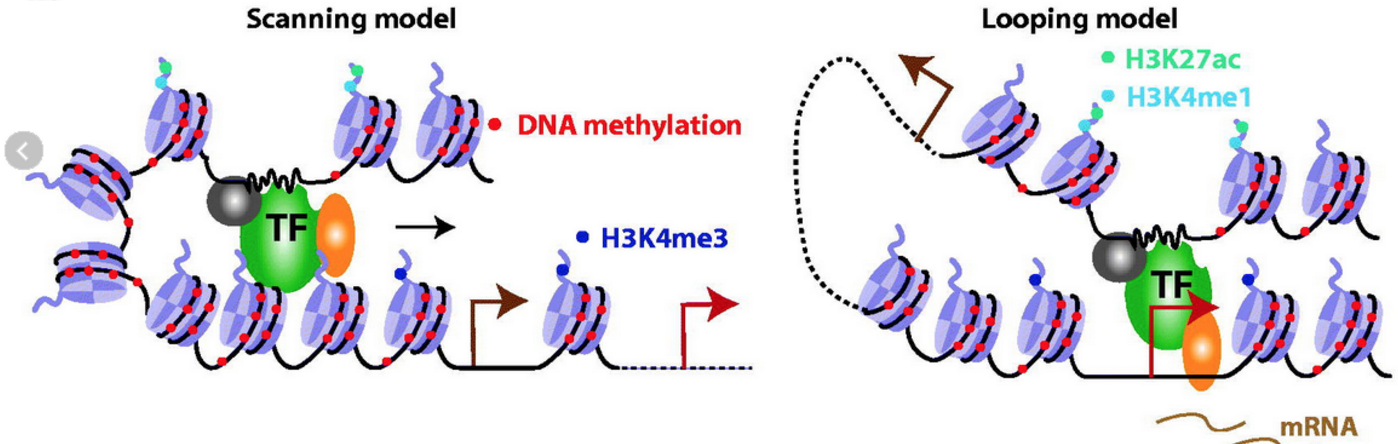
\includegraphics[width=1.0\linewidth]{ELMER/elmer.png}{\tiny{\\\href{https://genomebiology.biomedcentral.com/articles/10.1186/s13059-015-0668-3}{Yao et al. Genome Biology (2015) 16:105.}}}
 \end{figure}
 \pdfnote{\tiny{ scanning or tracking model: TF  binds at an enhancer and moves along the genome, searching for a target promoter }}
 \pdfnote{\tiny{  looping model:  enhancer directly interacts with a target promoter by forming a DNA loop }}

\end{frame}



\begin{frame}{Enhancer-mediated gene regulation}
 \begin{itemize}
  \item 73\% of the tested distal elements do not link to the nearest gene (Sanyal et al., 2012)
  \item 40\% of the enhancers involved in loops do not interact with the TSS of the nearest gene (Li et al., 2012),
  \item one-third of the distal interactions were not directed to the promoter of the nearest gene (Mifsud et al., 2015),
  \item 85\% of tumor-specific enhancers that could be linked to the expression of a nearby gene skipped the nearest gene (Yao et al., 2015).
 \end{itemize}
\end{frame}

\begin{frame}{ Enhancer-mediated gene regulation}
 \vspace*{-0.1cm}
 \begin{figure}
  \centering
  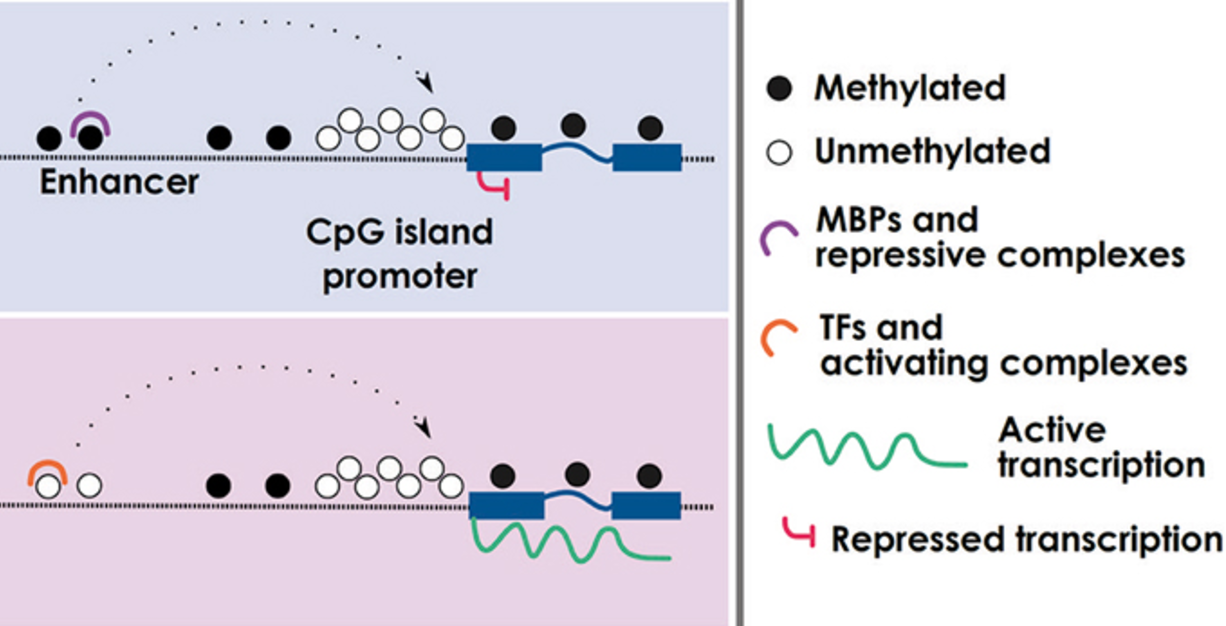
\includegraphics[width=1.0\linewidth]{dna_met.png}{\tiny{\\Source: Front. Aging Neurosci., 05 March 2015 http://dx.doi.org/10.3389/fnagi.2015.00019.}}
 \end{figure}
\end{frame}

\begin{frame}{ Enhancer Linking by Methylation/Expression Relationship}
 \vspace*{-0.5cm}
 \begin{figure}
  \centering
  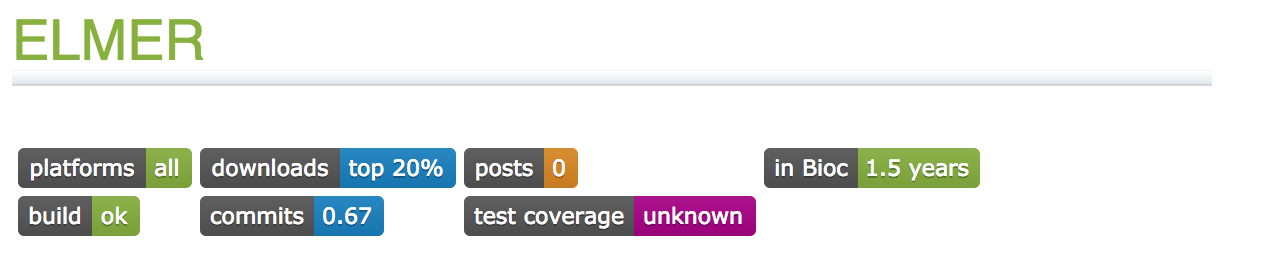
\includegraphics[width=0.8\linewidth]{ELMER/elmer1.png}
 \end{figure}
 \vspace*{-0.5cm}
 \begin{figure}
  \centering
  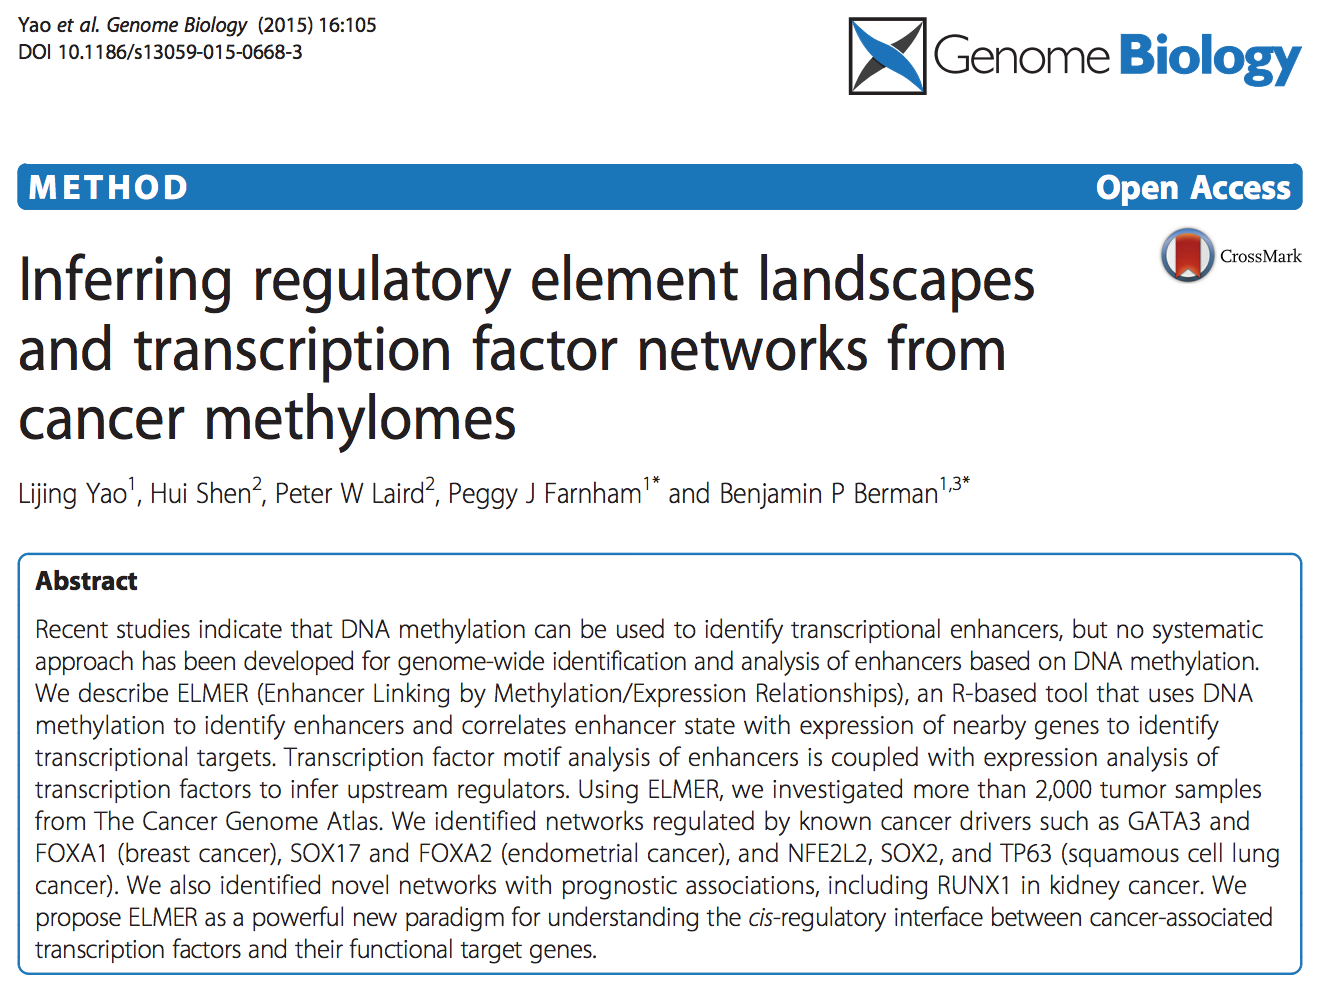
\includegraphics[width=0.8\linewidth]{ELMER/elmer2.png}
 \end{figure}
\end{frame}



\begin{frame}[plain]%{Workflow}
 \vspace*{-0.3cm}
 \begin{figure}
  \centering
  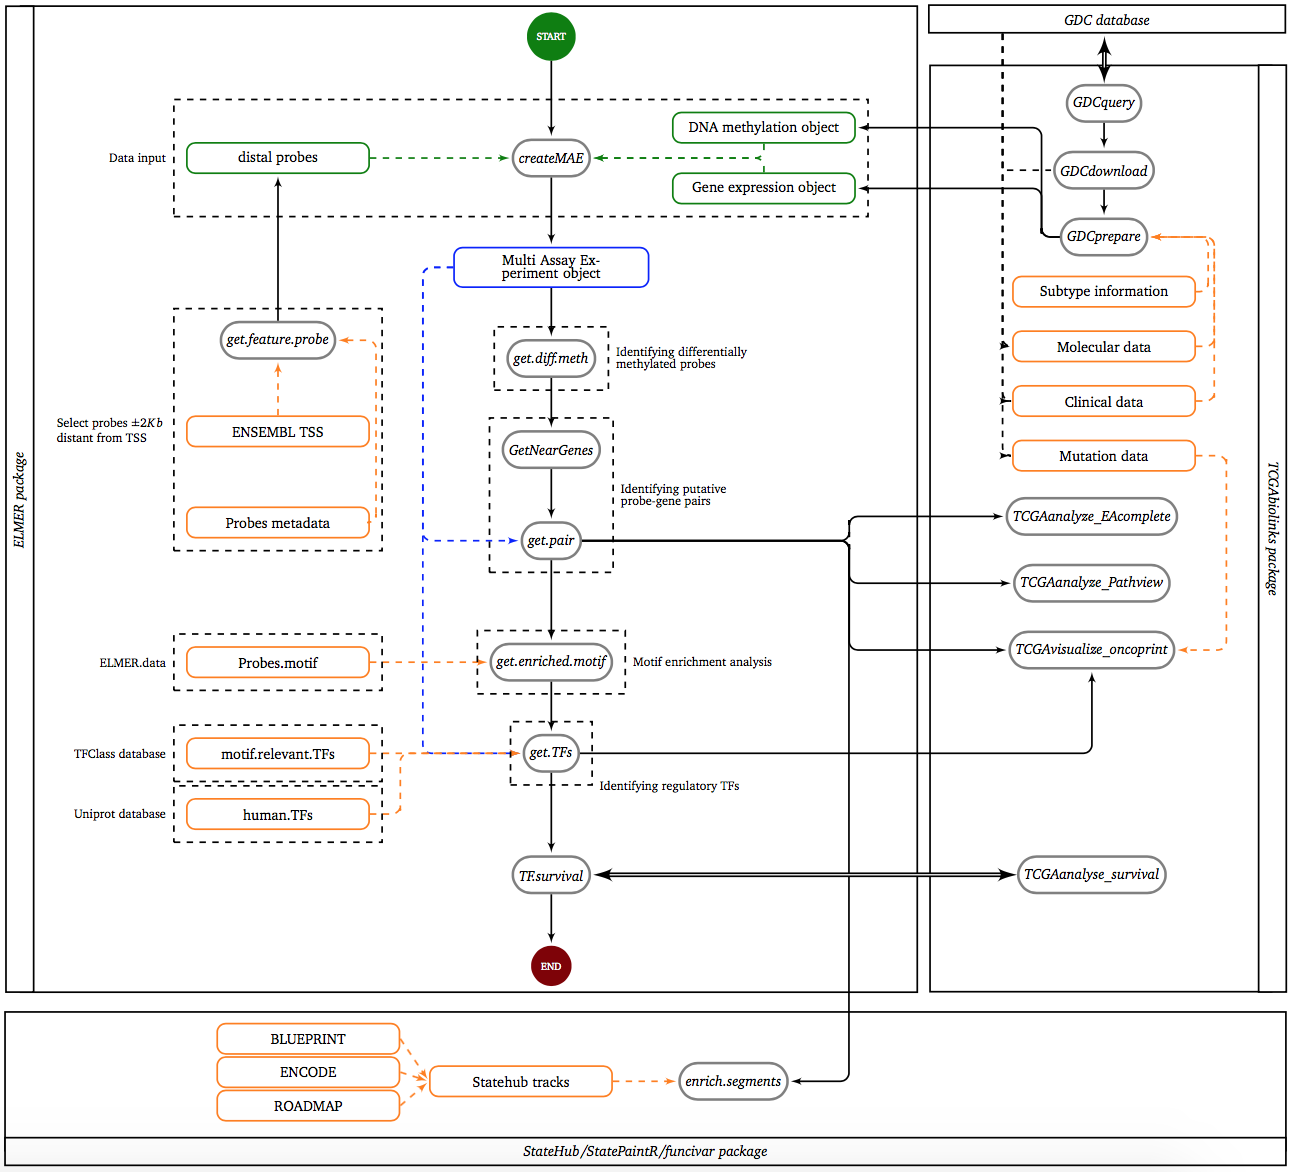
\includegraphics[width=0.95\linewidth]{workflow_elmer2.png}
 \end{figure}
\end{frame}


%\begin{frame}{Algorithm}

%\begin{exampleblock}{Steps}
%\begin{enumerate}
%\item  Identify distal  probes on HM450K/EPIC.
%\item  Identify distal  probes with significantly different DNA methylation level in  group 1 compared to group 2.
%\item  Identify putative target genes for differentially methylated distal enhancer probes.
%\item  Identify enriched motifs for the distal  probes which are significantly differentially methylated and linked to putative target gene.
%\item  Identify regulatory TFs whose expression associate with DNA methylation at motifs.
%\end{enumerate}

%\end{exampleblock}


%\end{frame}


\begin{frame}{Step 1: Identify distal probes}
 %\vspace*{1.0cm}
 \begin{figure}
  \centering
  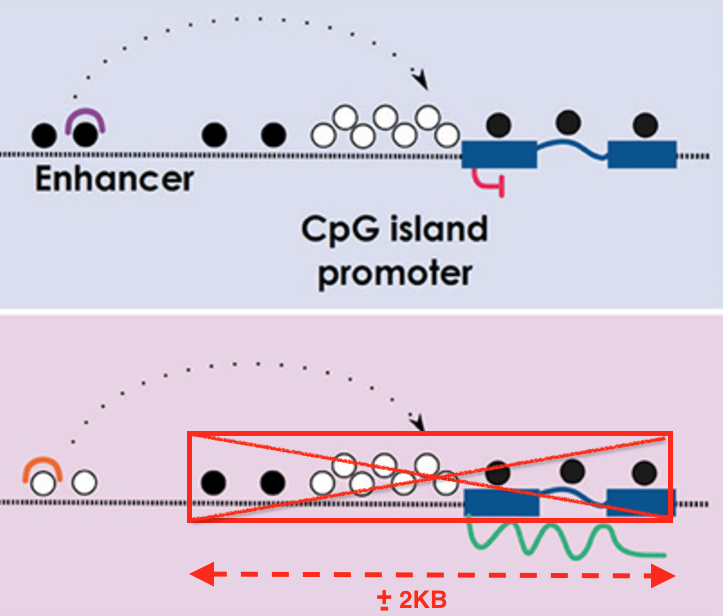
\includegraphics[width=0.7\linewidth]{step1.png}
 \end{figure}
\end{frame}


\begin{frame}{Step 2: Differentially methylated distal probes}
 \vspace*{-0.3cm}
 \begin{figure}
  \centering
  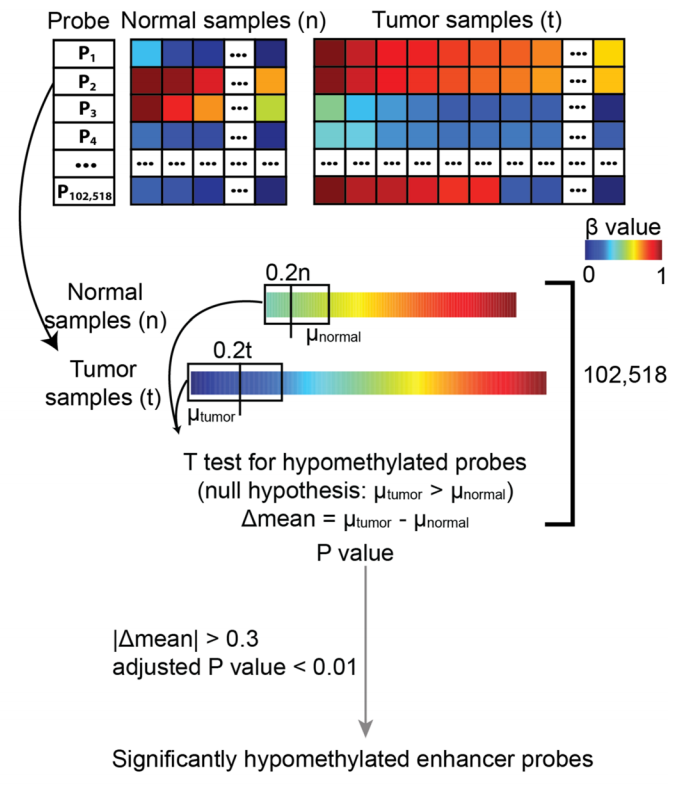
\includegraphics[width=0.5\linewidth]{diffmeth.png}{\tiny{\\Yao et al. Genome Biology (2015) 16:105.}}
 \end{figure}
\end{frame}

\begin{frame}{Step 2: Differentially methylated distal probes}
 \begin{figure}
  \centering
  \includegraphics[width=1.0\linewidth]{ELMER/volcano_plot.pdf}
 \end{figure}
\end{frame}

\begin{frame}{Step 2: Differentially methylated distal probes}
 \begin{figure}
  \centering
  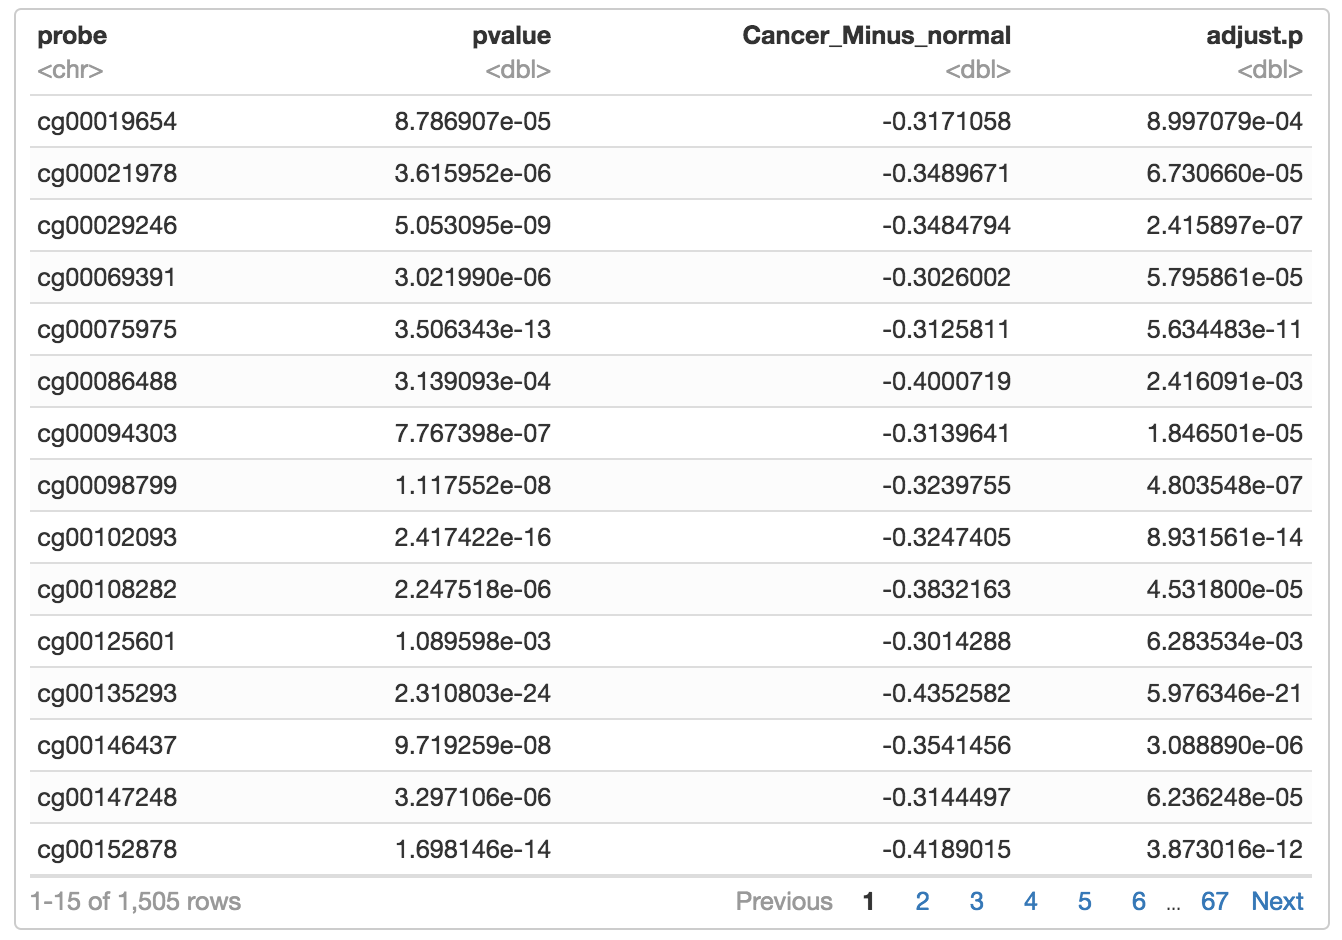
\includegraphics[width=0.9\linewidth]{ELMER/metdiff_tbl.png}
 \end{figure}
\end{frame}

\begin{frame}{Step 3: Get pairs}
 \vspace*{-0.3cm}
 \begin{figure}
  \centering
  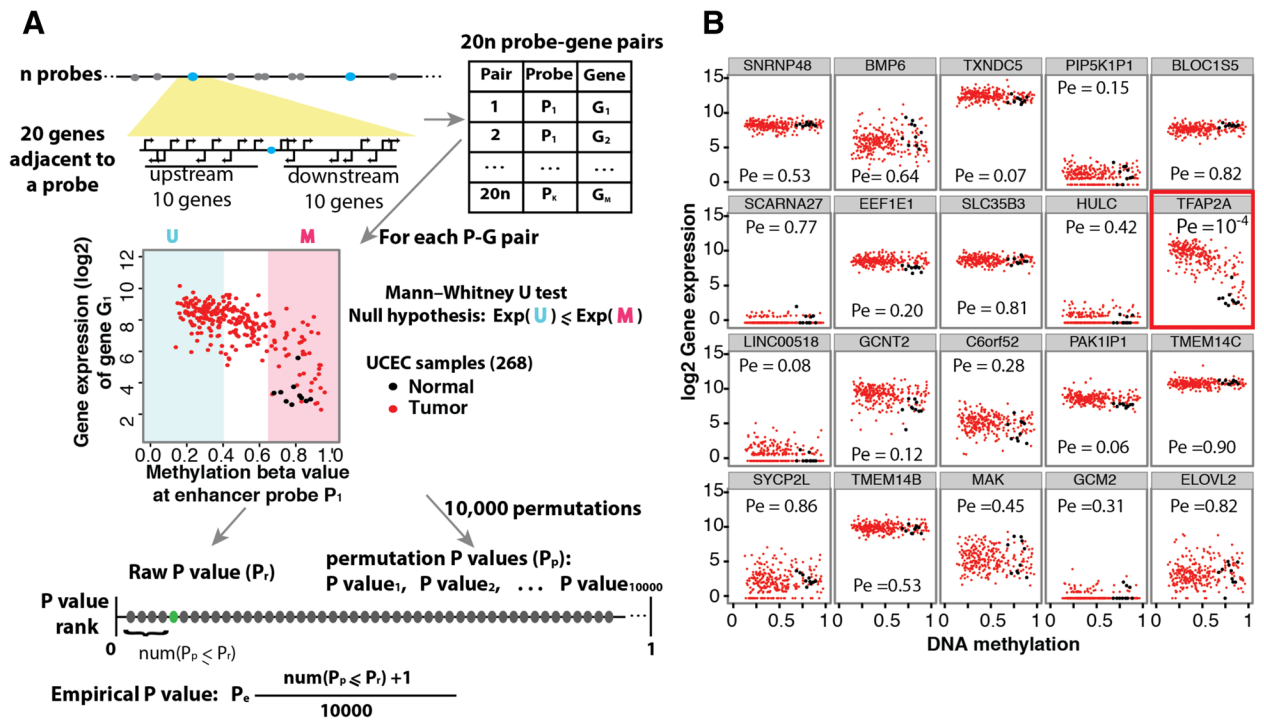
\includegraphics[width=1.0\linewidth]{ELMER/pair.png}{\tiny{\\Yao et al. Genome Biology (2015) 16:105.}}
 \end{figure}
\end{frame}



\begin{frame}{Step 3: Pairs inferred}
 \begin{figure}
  \centering
  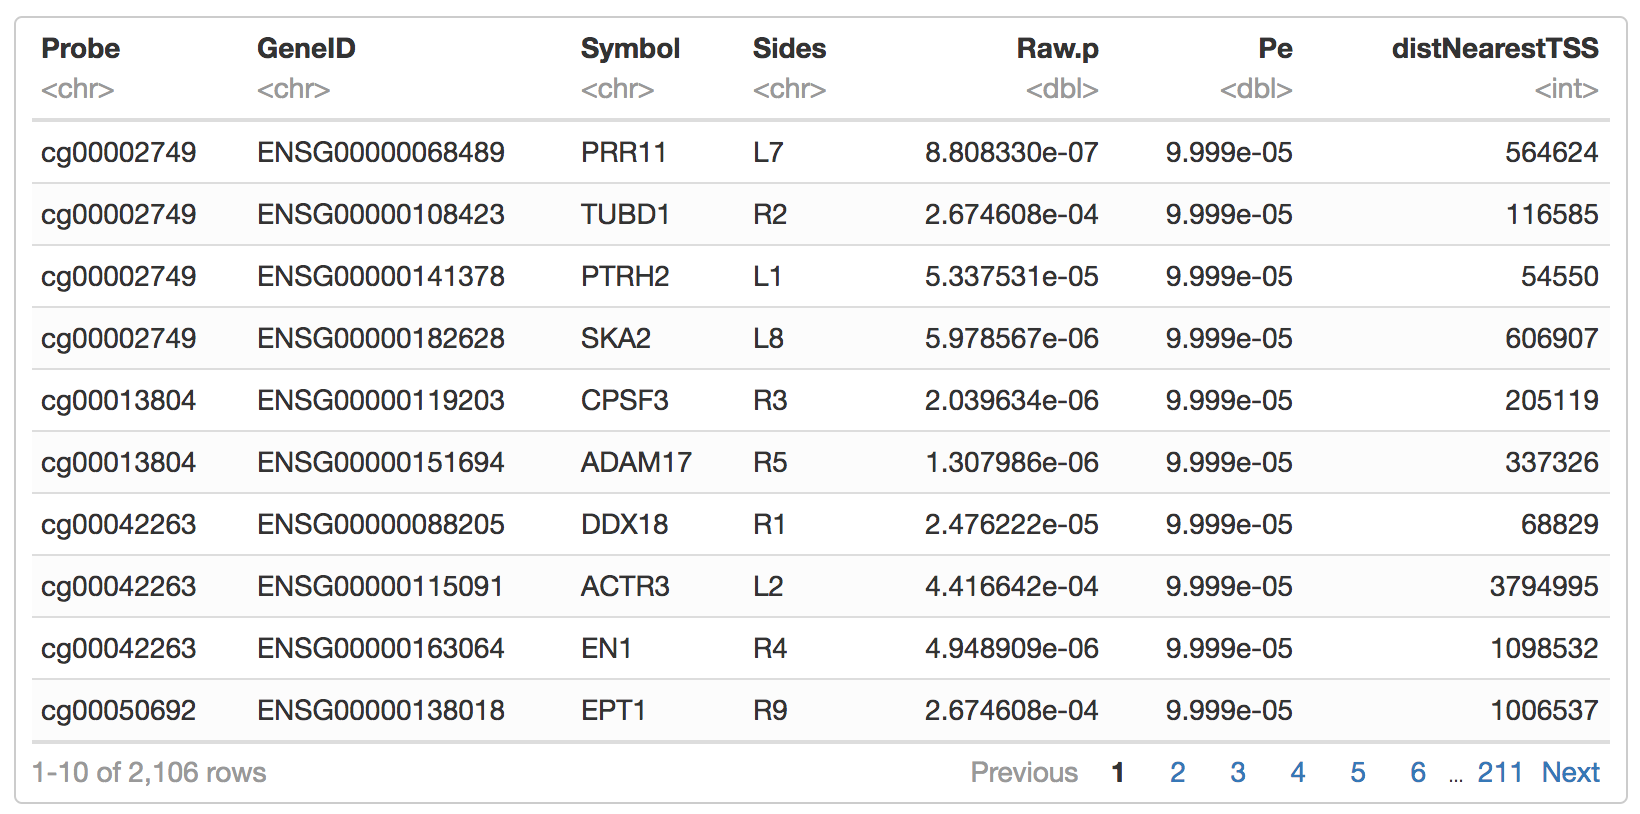
\includegraphics[width=1.0\linewidth]{ELMER/pairs_tbl.png}
 \end{figure}
\end{frame}

\begin{frame}{Step 3: Pairs inferred}
 \vspace*{-0.3cm}
 \begin{figure}
  \centering
  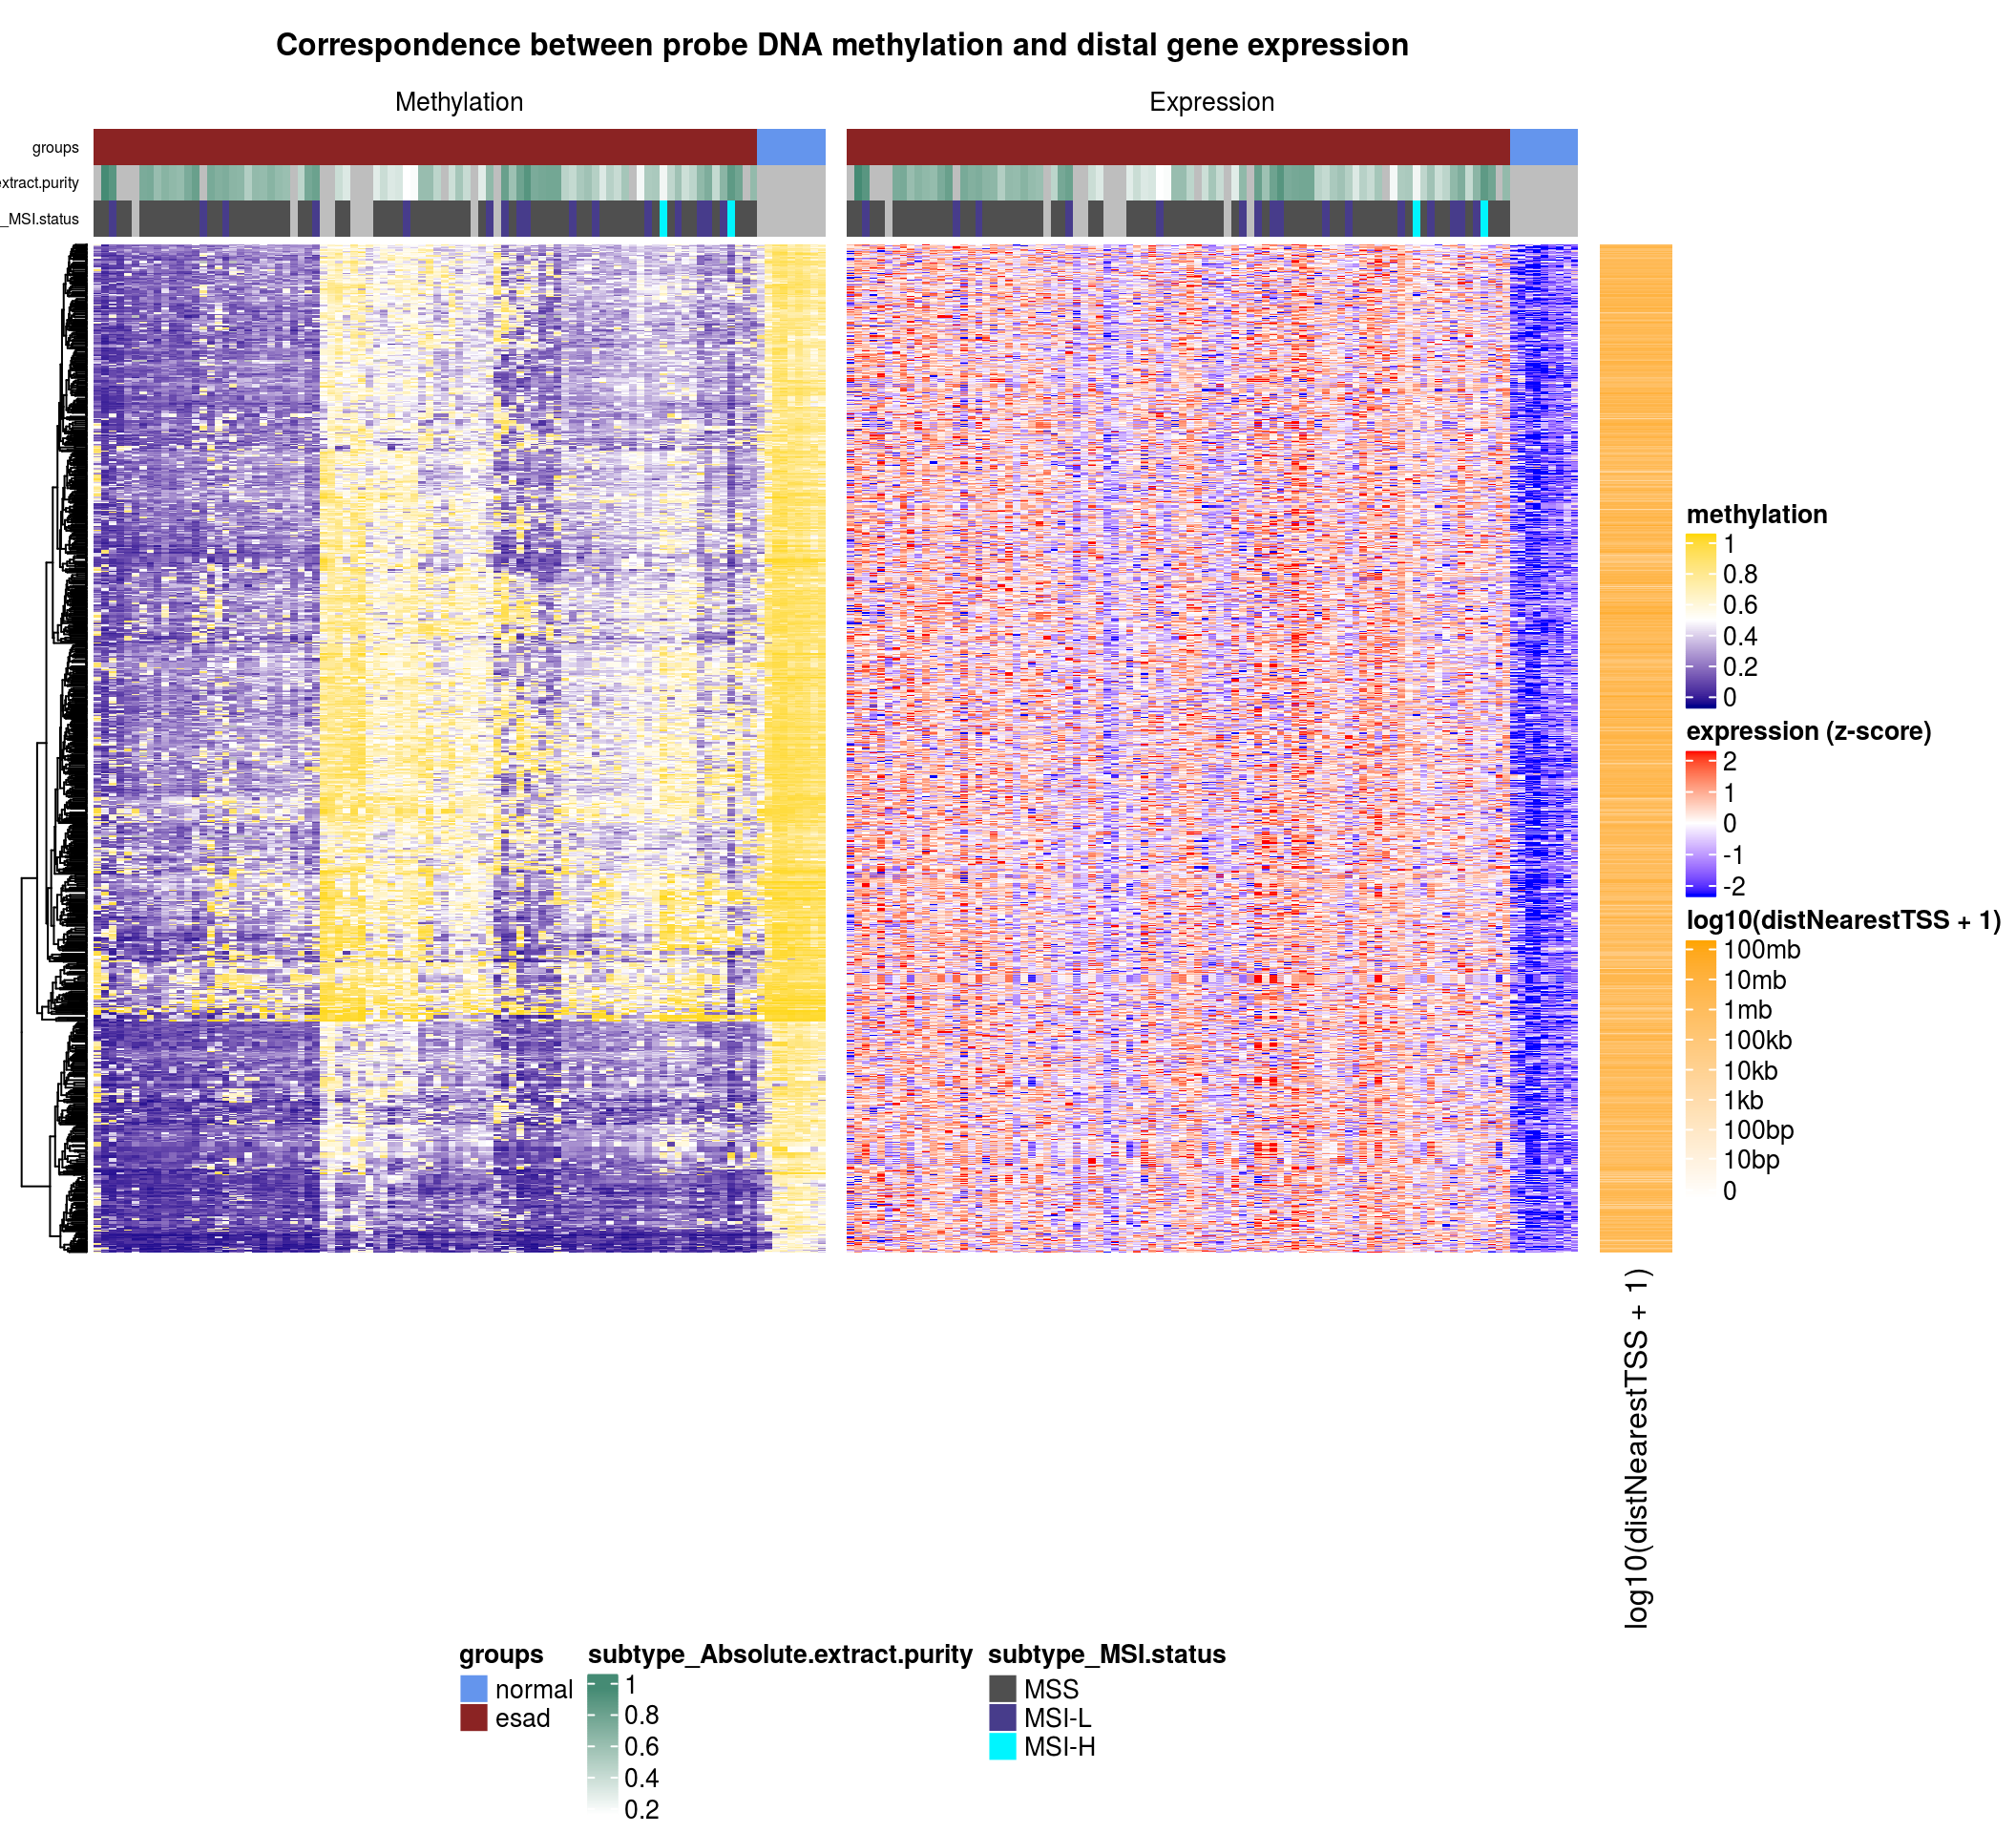
\includegraphics[width=0.75\linewidth]{ELMER/heatmappair.png}
 \end{figure}
\end{frame}


\begin{frame}{Step 4: Enriched motifs}

 \vspace*{-0.3cm}
 \begin{figure}
  \centering
  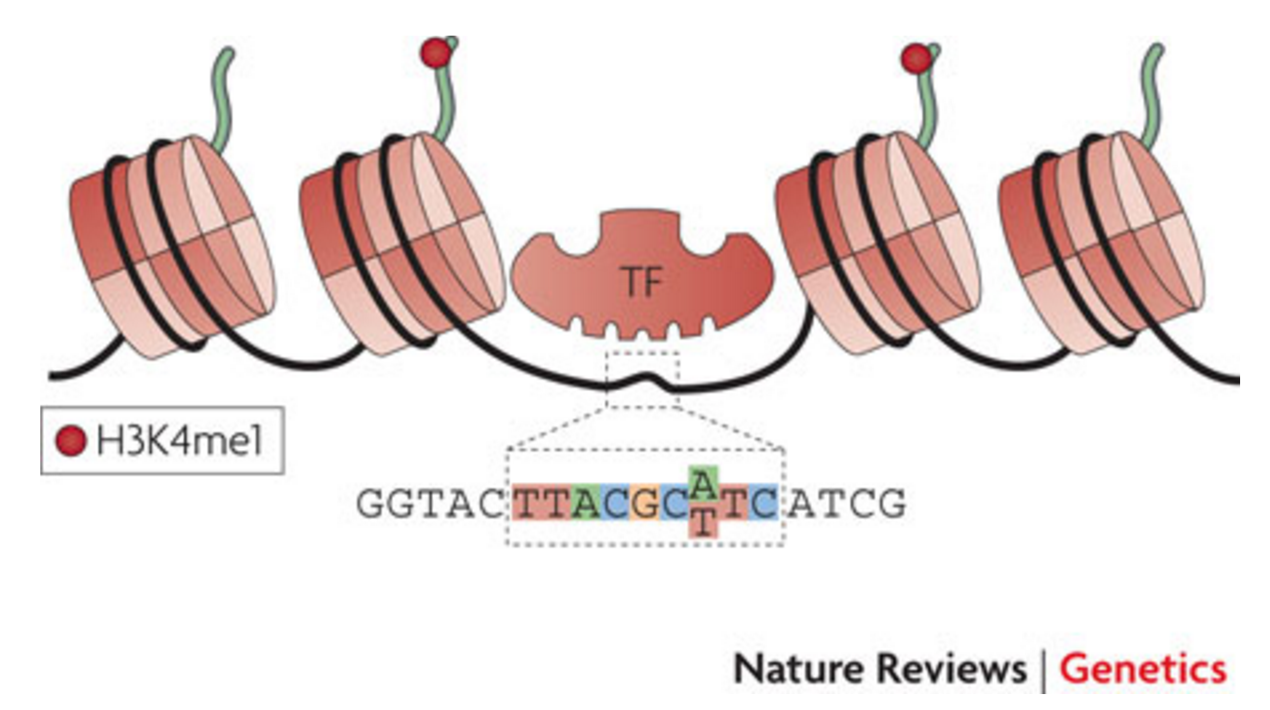
\includegraphics[width=1.0\linewidth]{ELMER/tf_binding.png}{\tiny{\\Next-generation genomics: an integrative approach R. David Hawkins et al. Nature Reviews Genetics 11, 476-486}}
 \end{figure}
\end{frame}


\begin{frame}{Step 4:  Enriched motifs}
 \vspace*{-0.3cm}
 \begin{figure}
  \centering
  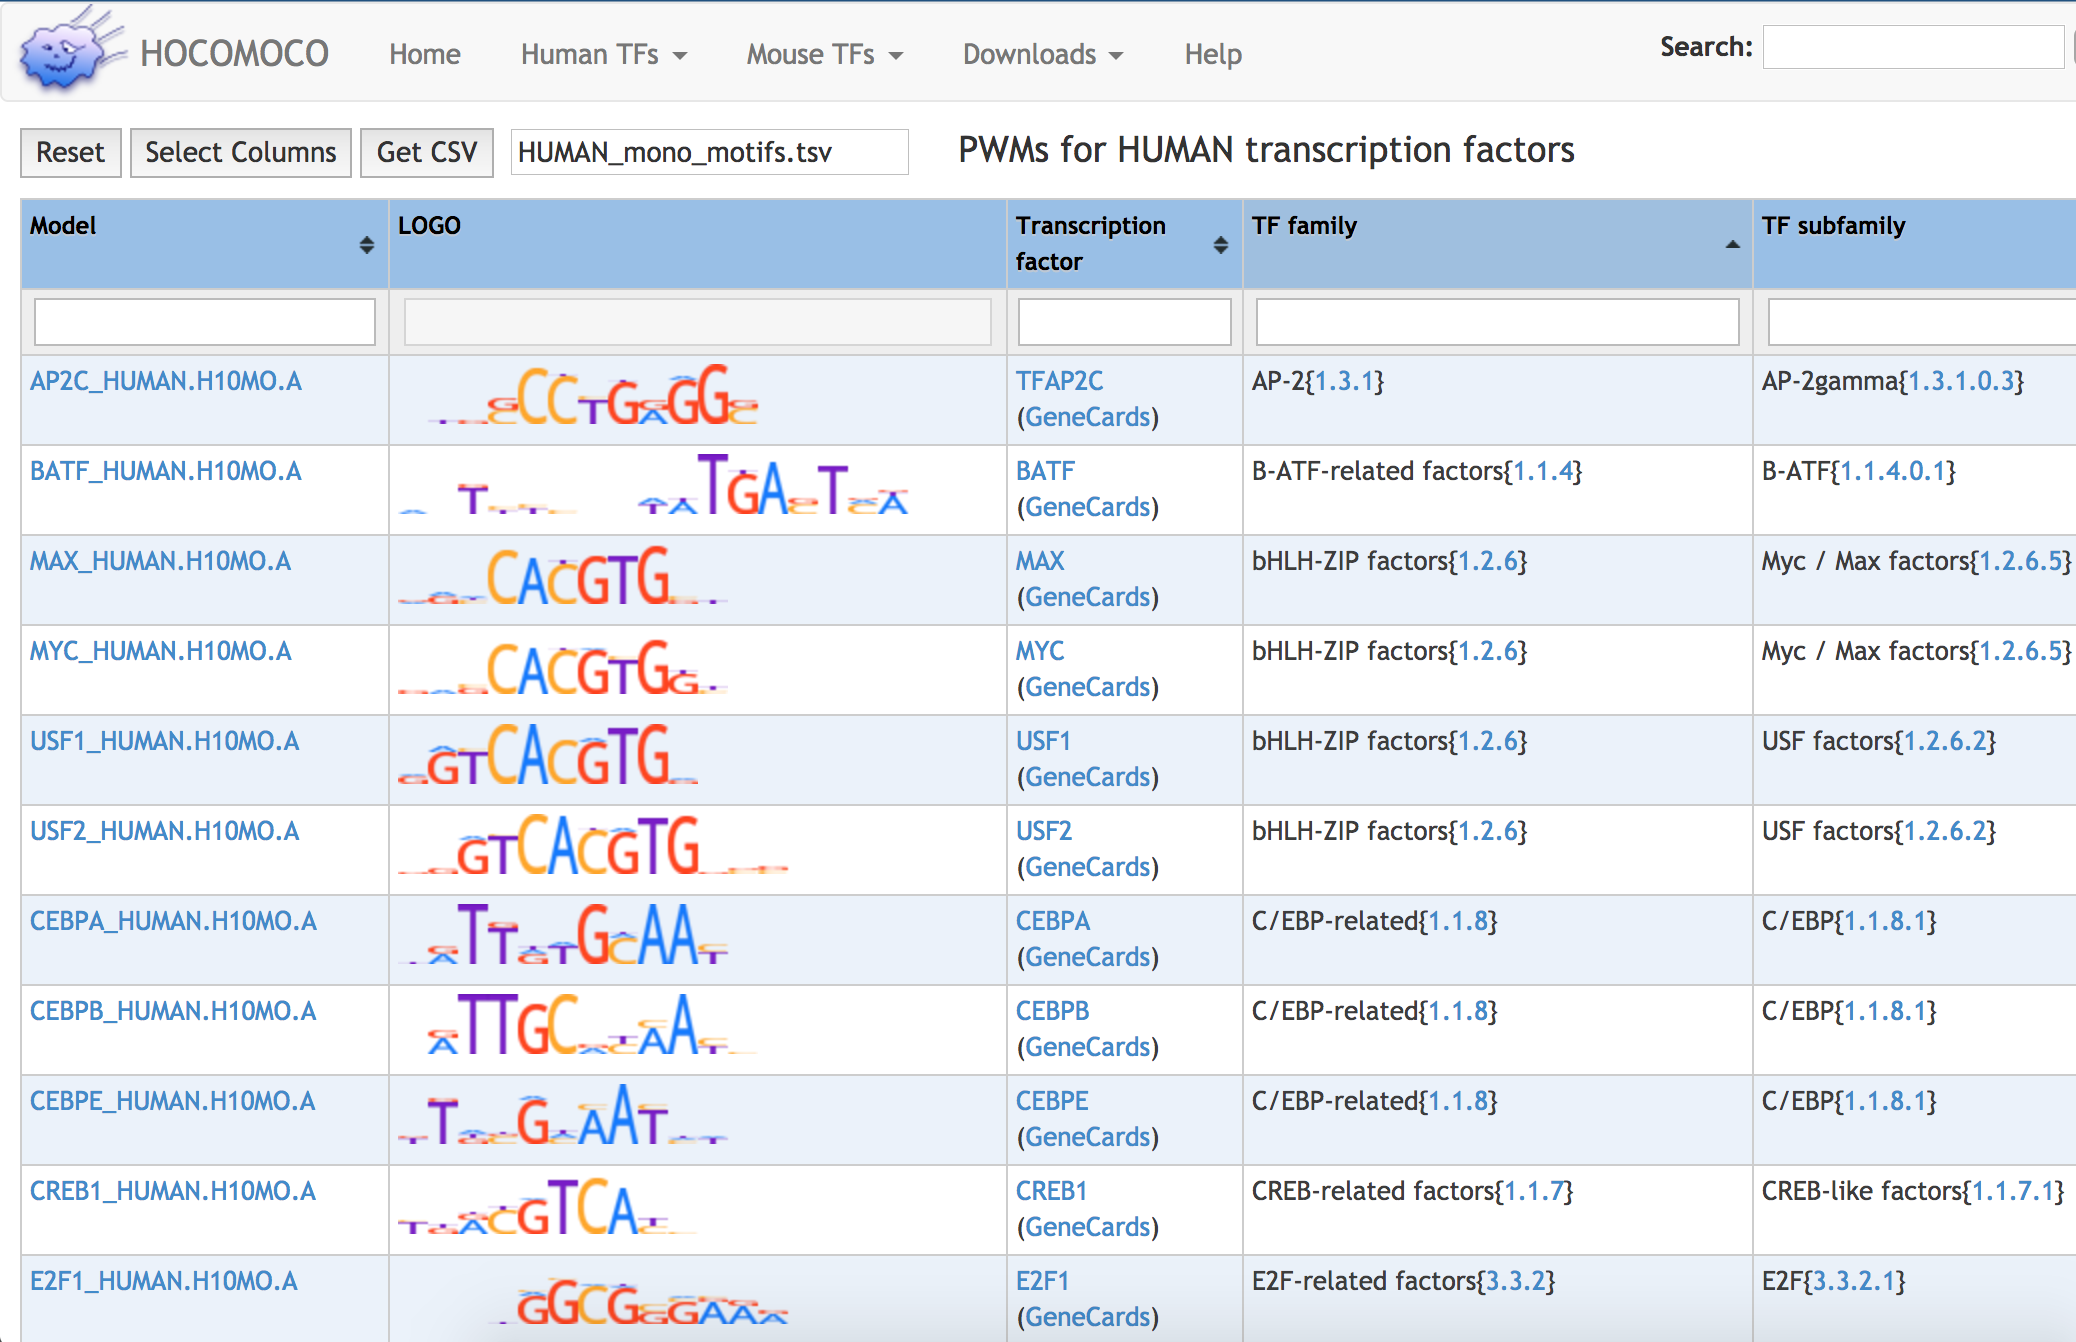
\includegraphics[width=1.0\linewidth]{hocomoco.png}
 \end{figure}
\end{frame}

\begin{frame}{Step 4: Motif Enrichment}

\begin{block}{Objective}
Evaluate the enrichment of transcription factors in certain genomic regions.
\begin{enumerate}
  \item Perform motif matching of transcription factors in probes regions (window $\pm250bp$)
  \item Evaluate which transcription factors are more likely to occur in those regions than in background regions
  using Fisher’s exact test with FDR correction.
\end{enumerate}
\end{block}
 \begin{exampleblock}{Fisher’s exact test}
 a: nb of input regions with match for TF motif.\\
 b: nb of input regions with no match for TF motif.\\
 c: nb of background regions with match for TF motif.\\
 d: nb of background regions with no match for TF motif.
 \end{exampleblock}

\end{frame}

\begin{frame}{Step 4: Motif enrichment}
 \begin{figure}
  \centering
  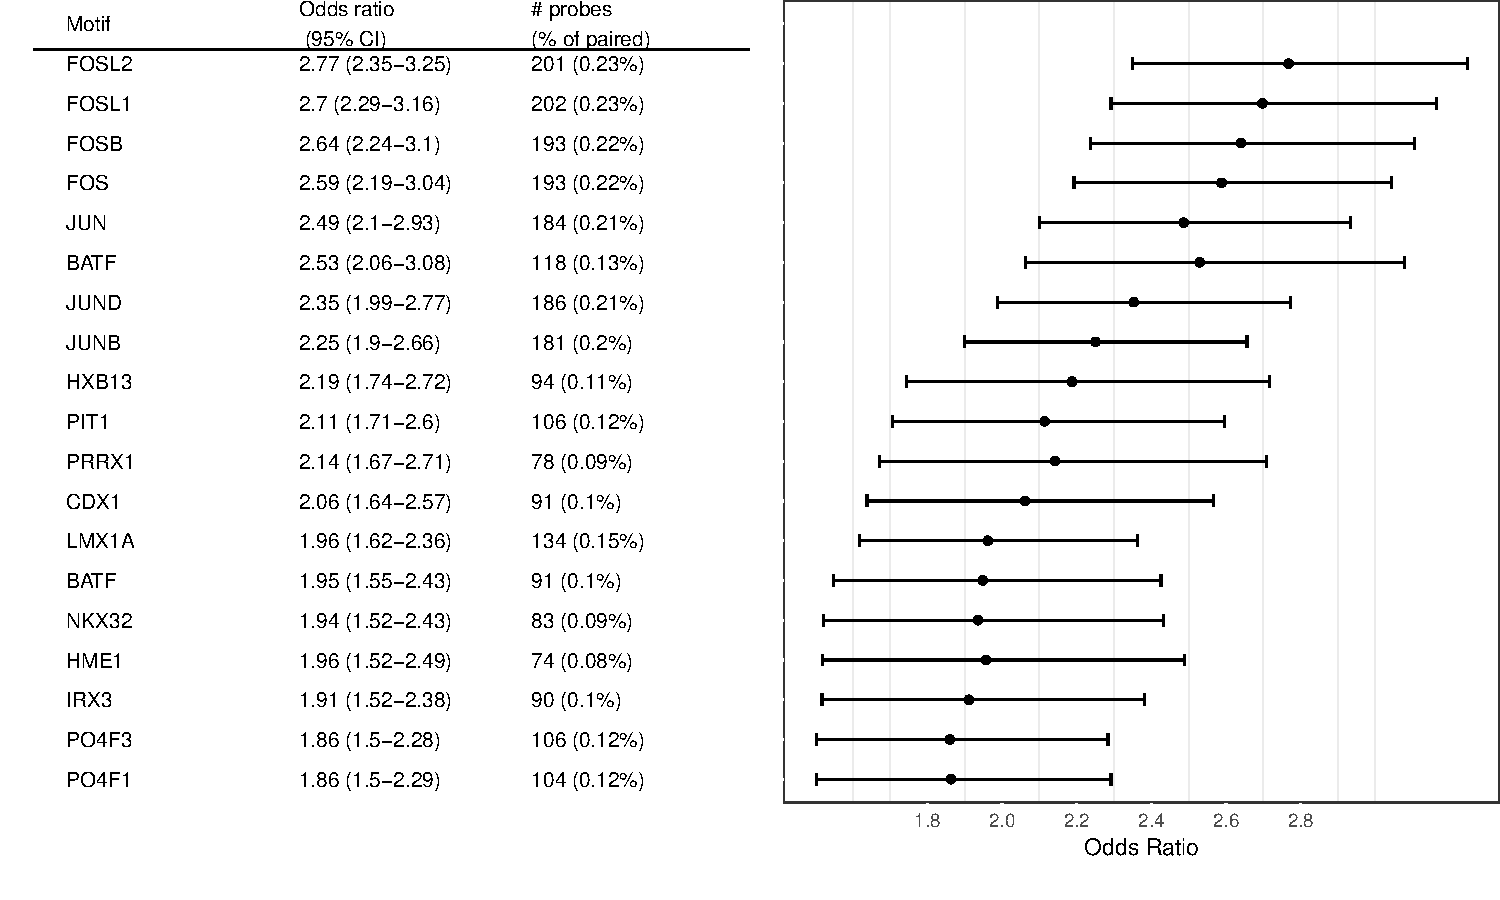
\includegraphics[width=1.0\linewidth]{ELMER/motif_enrichment.pdf}
 \end{figure}
\end{frame}

\begin{frame}{Step 4: Motif enrichment}
 \begin{figure}
  \centering
  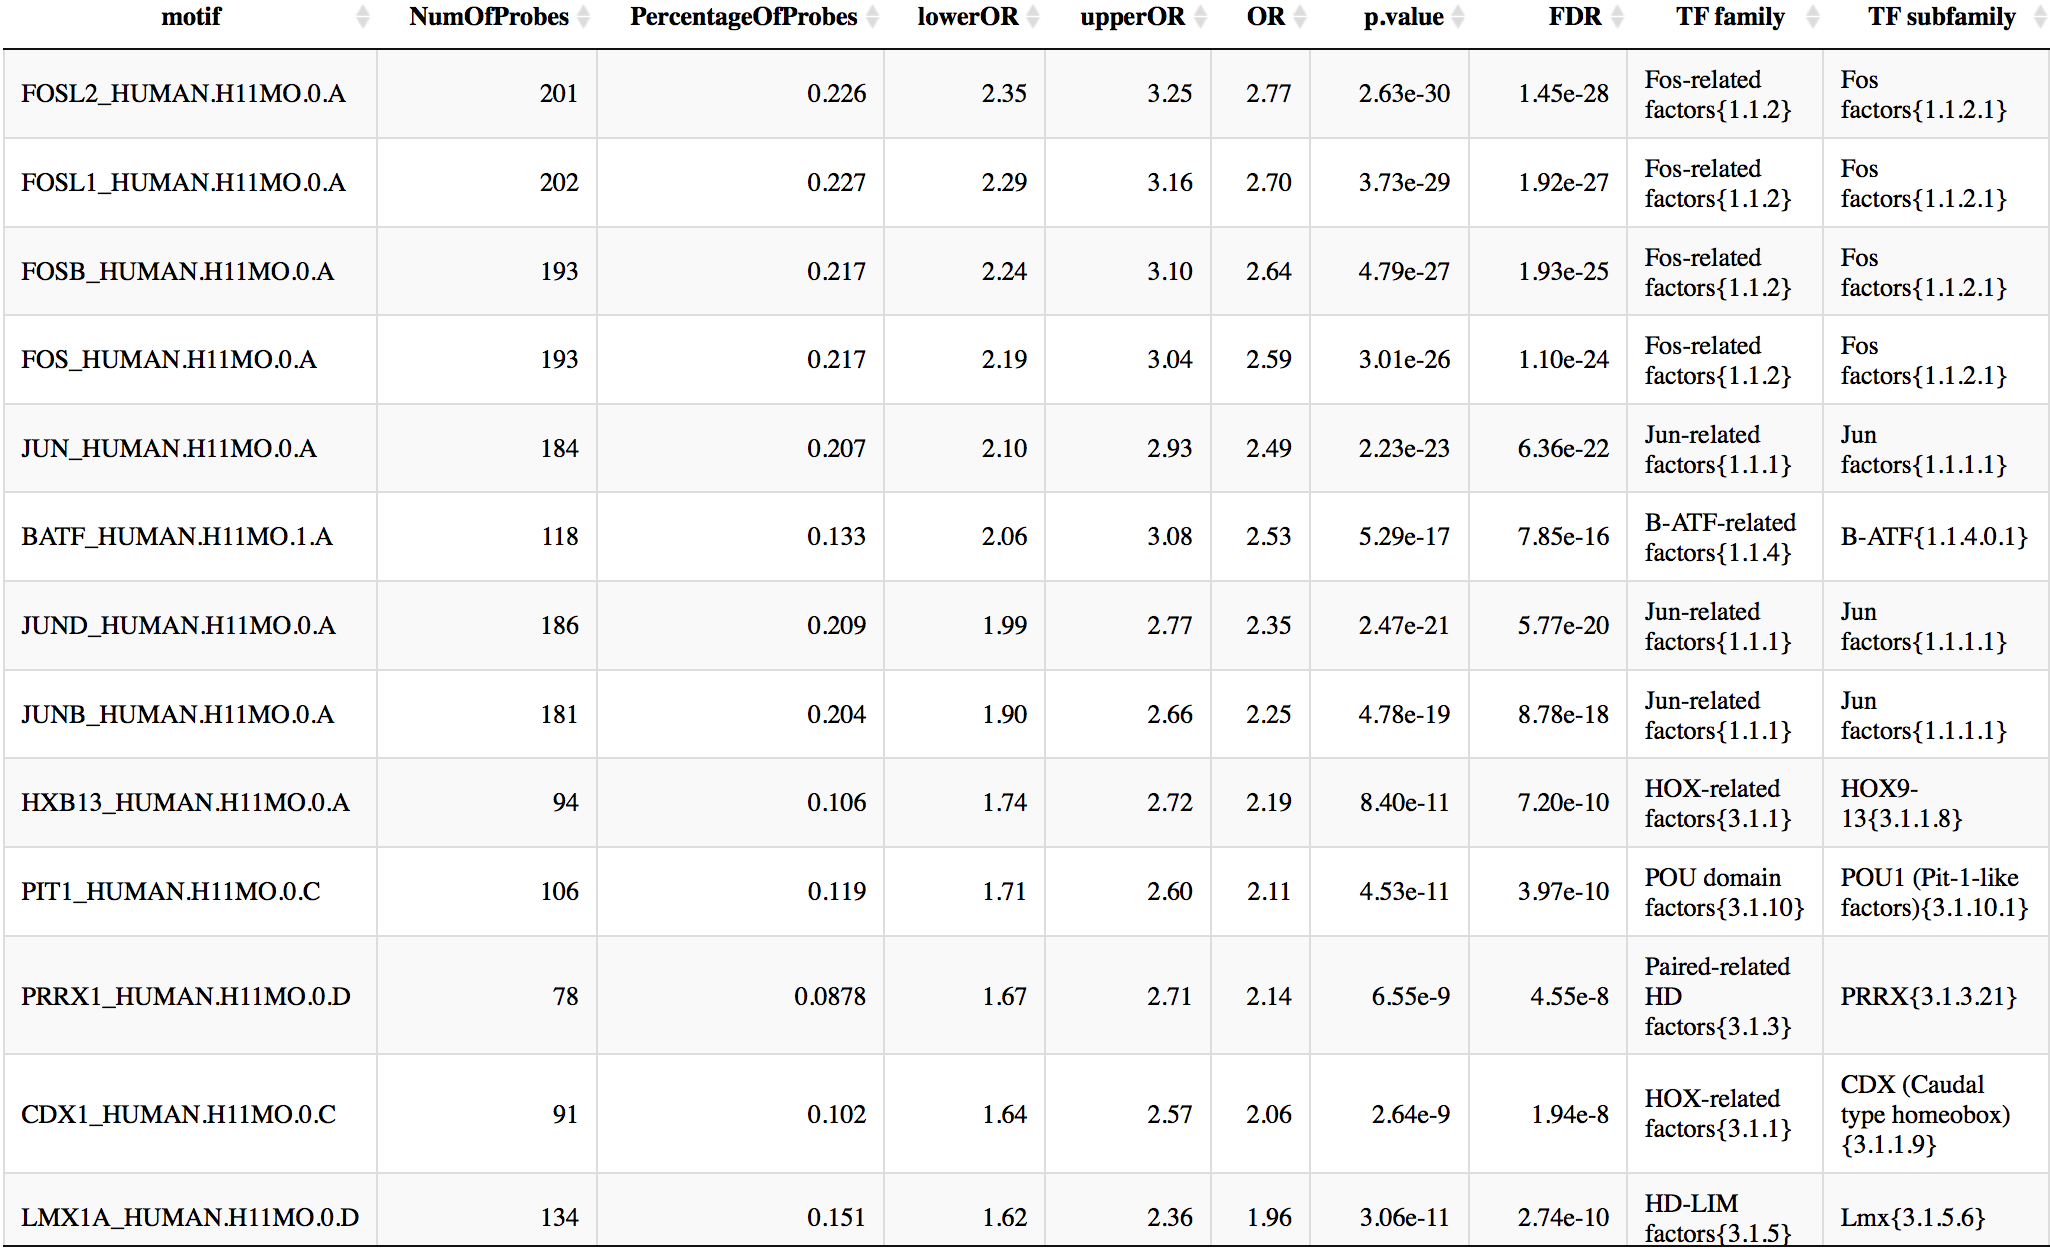
\includegraphics[width=1.0\linewidth]{ELMER/or_tbl.png}
 \end{figure}
\end{frame}


\begin{frame}{Step 5: Human TFs}
 \vspace*{-0.3cm}
 \begin{figure}
  \centering
  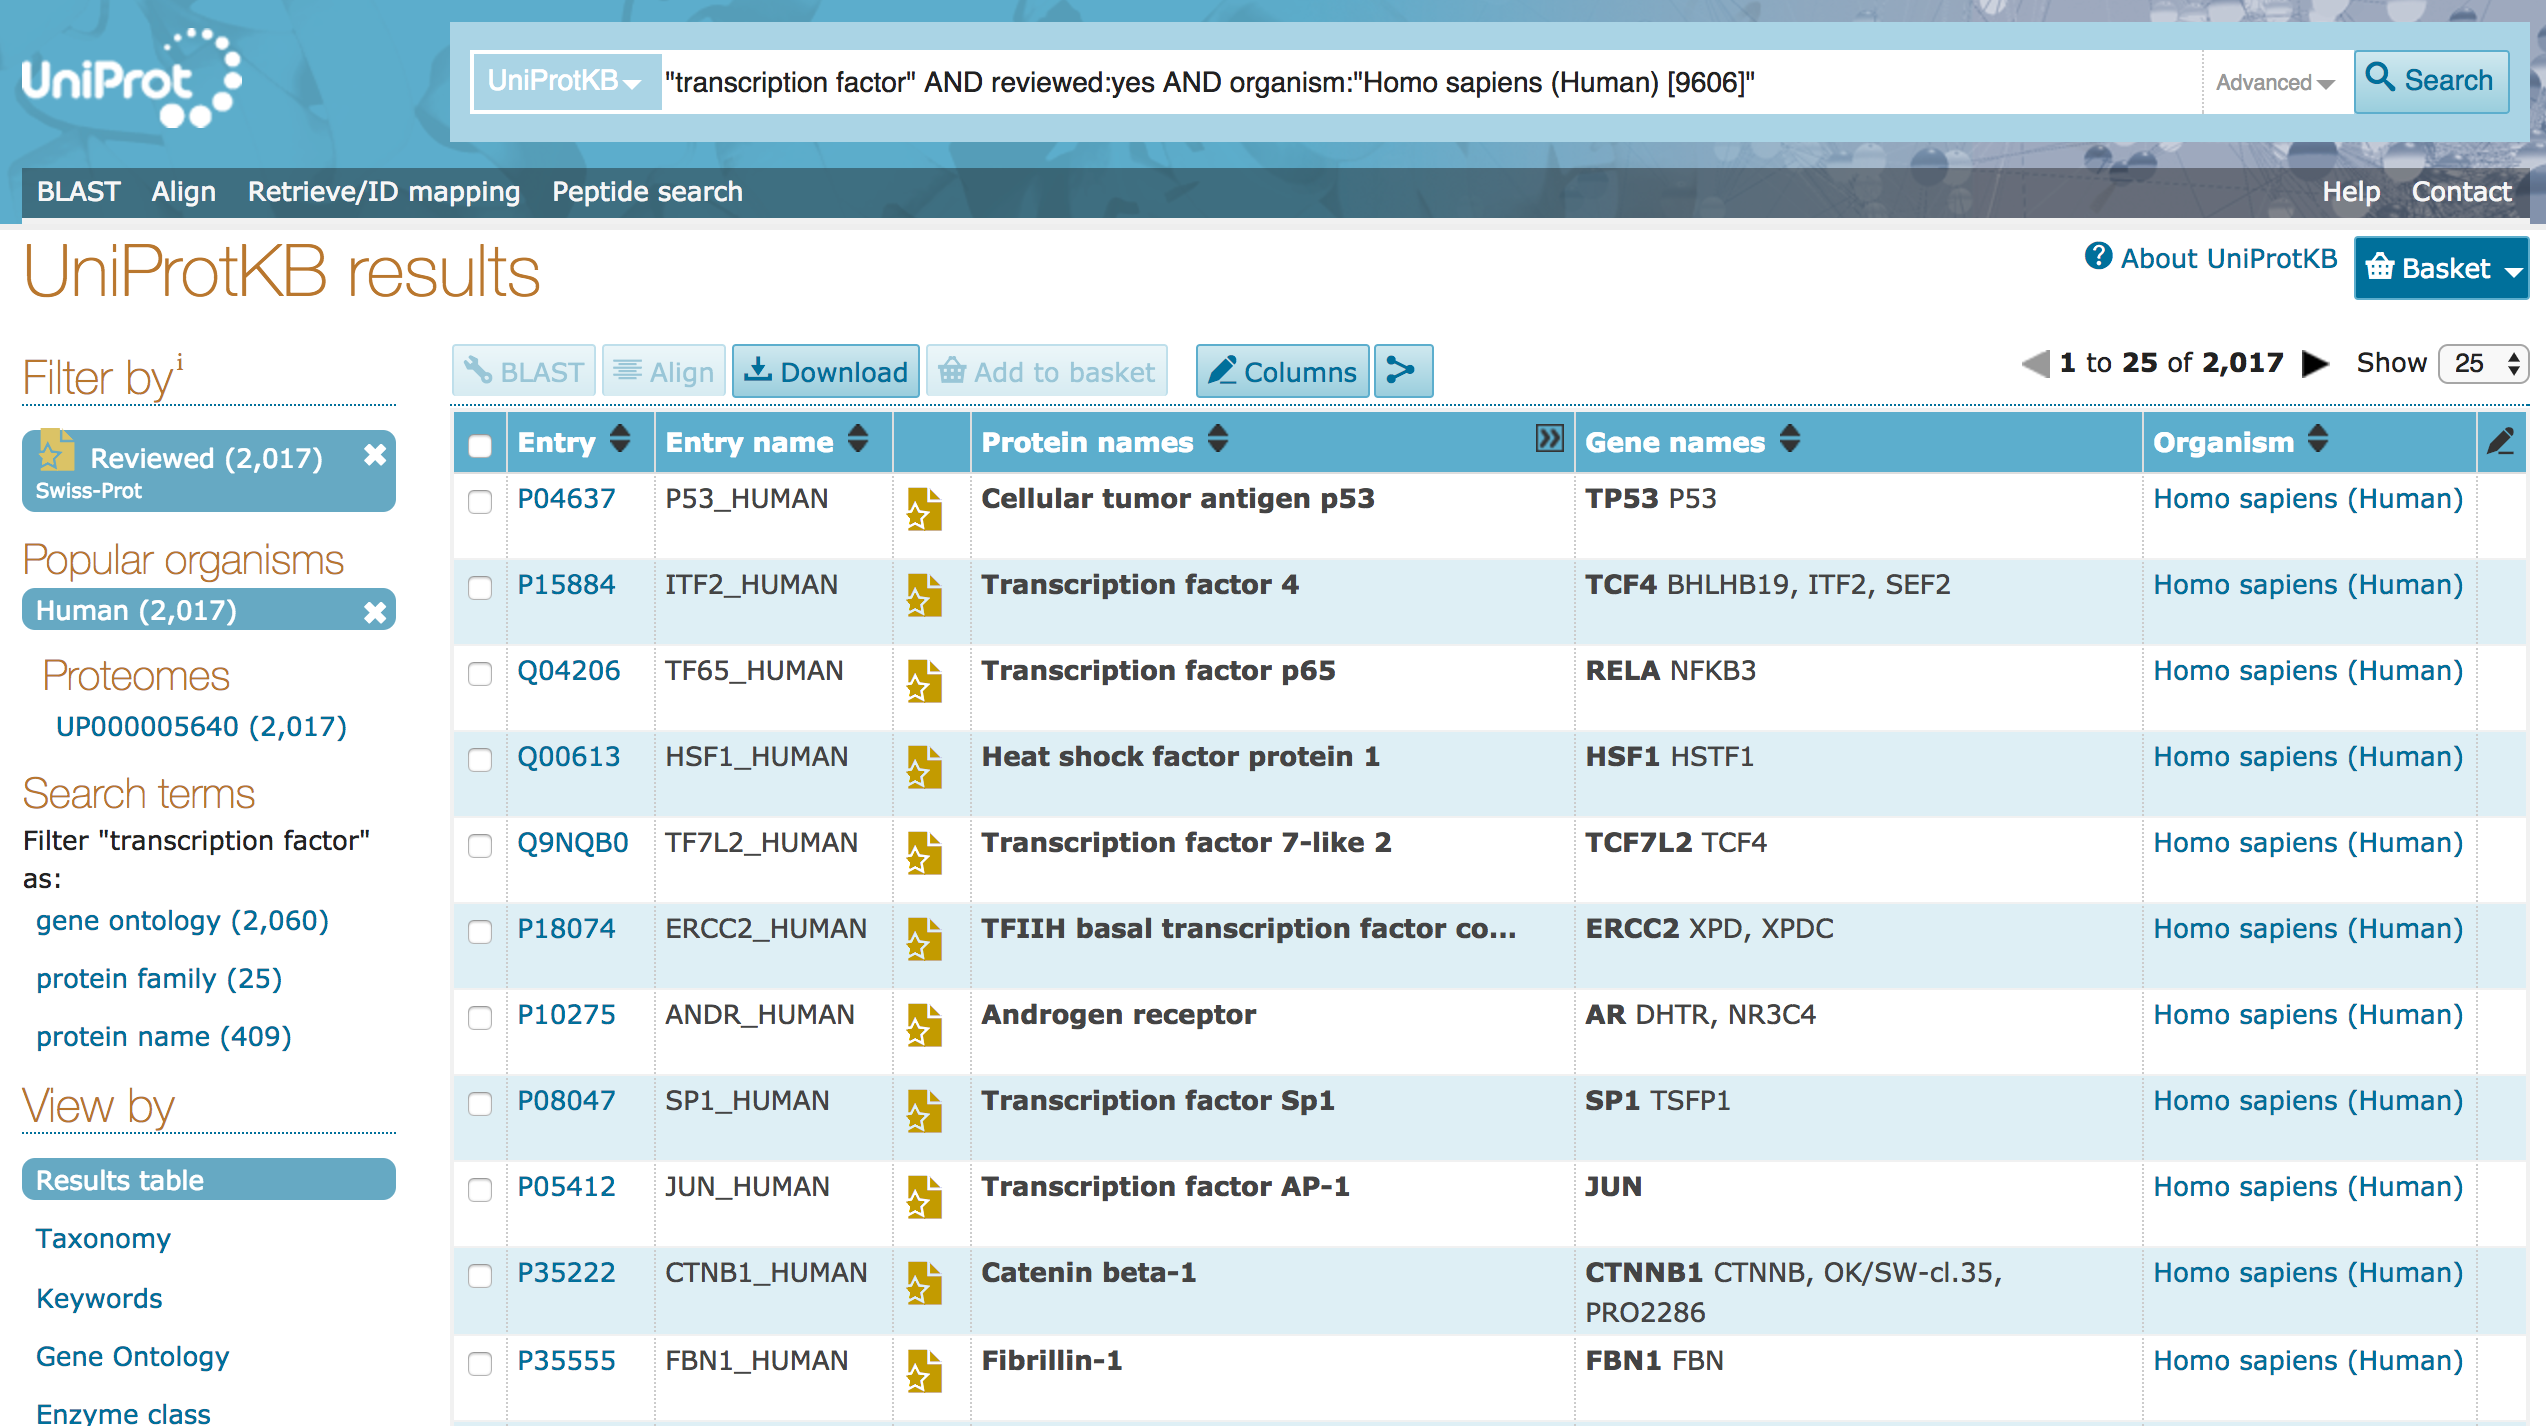
\includegraphics[width=1.0\linewidth]{ELMER/uniprot.png}
 \end{figure}
\end{frame}

\begin{frame}{Step 5: Identification of master regulator TF}
 \vspace*{-0.5cm}
 \begin{figure}
  \centering
  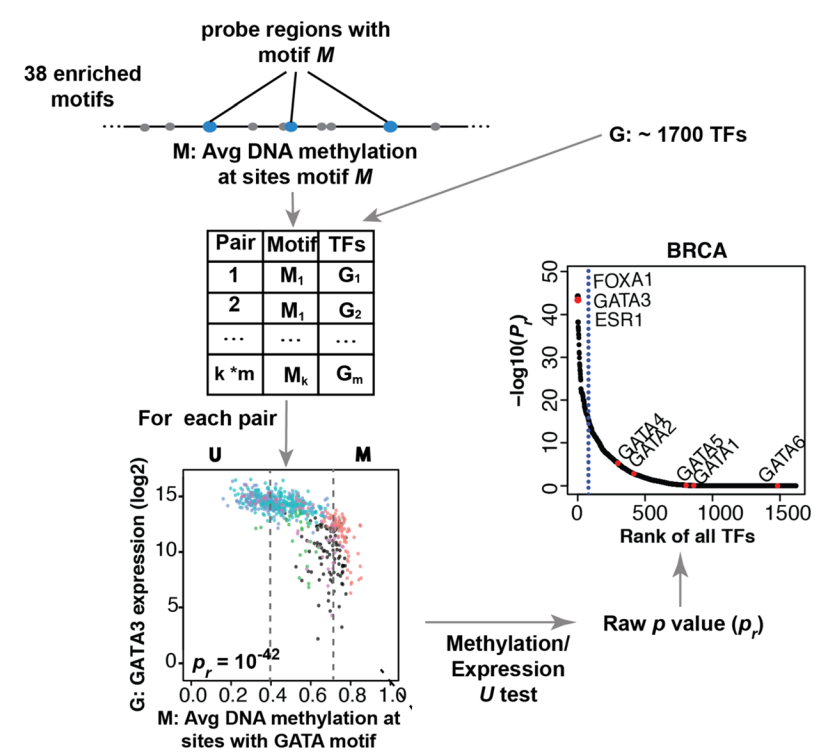
\includegraphics[width=0.7\linewidth]{ELMER/tfrank.png}{\tiny{\\\href{https://genomebiology.biomedcentral.com/articles/10.1186/s13059-015-0668-3}{Yao et al. Genome Biology (2015) 16:105.}}}
 \end{figure}
\end{frame}

\begin{frame}{Step 5: TF ranking plot}
 \begin{figure}
  \centering
  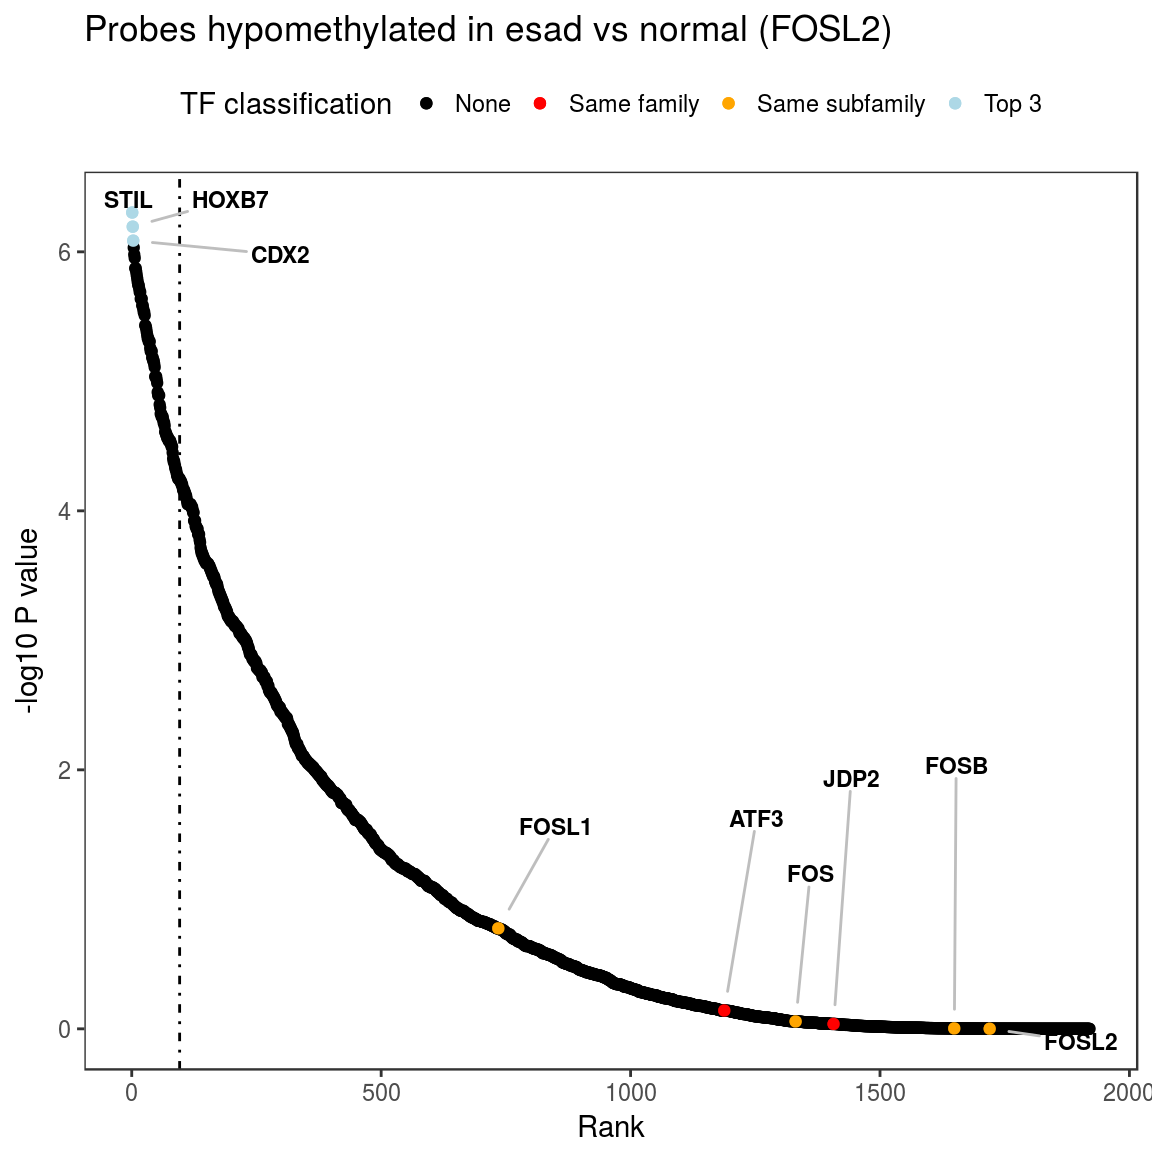
\includegraphics[width=0.45\linewidth]{ELMER/FOS_TF.png}
  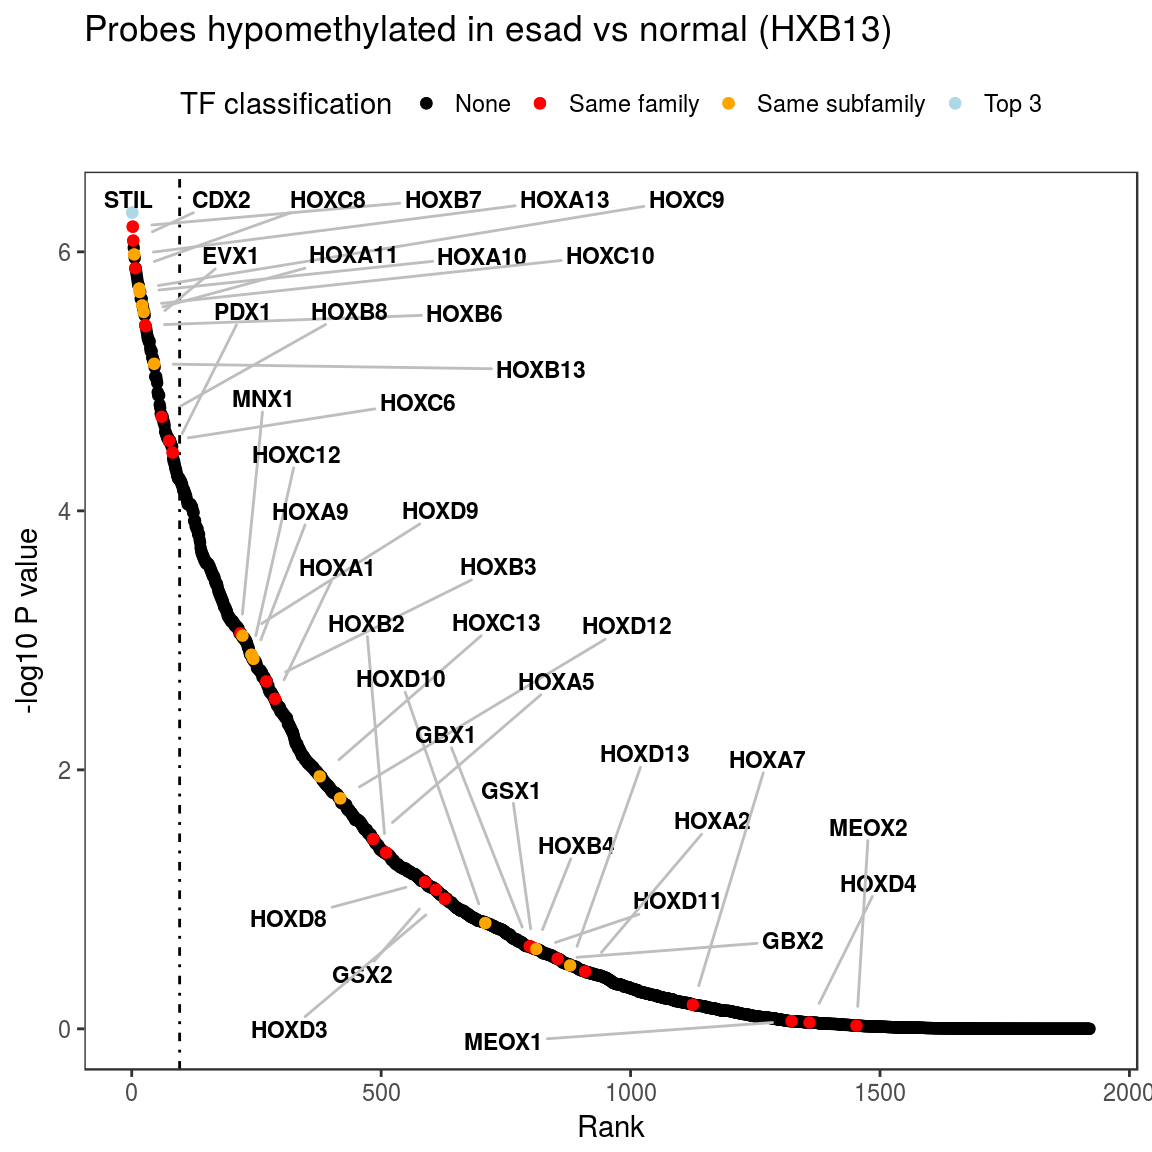
\includegraphics[width=0.45\linewidth]{ELMER/HOX_TF.png}
 \end{figure}
\end{frame}

\begin{frame}{Step 5: TF scatter plot}
 \begin{figure}
  \centering
  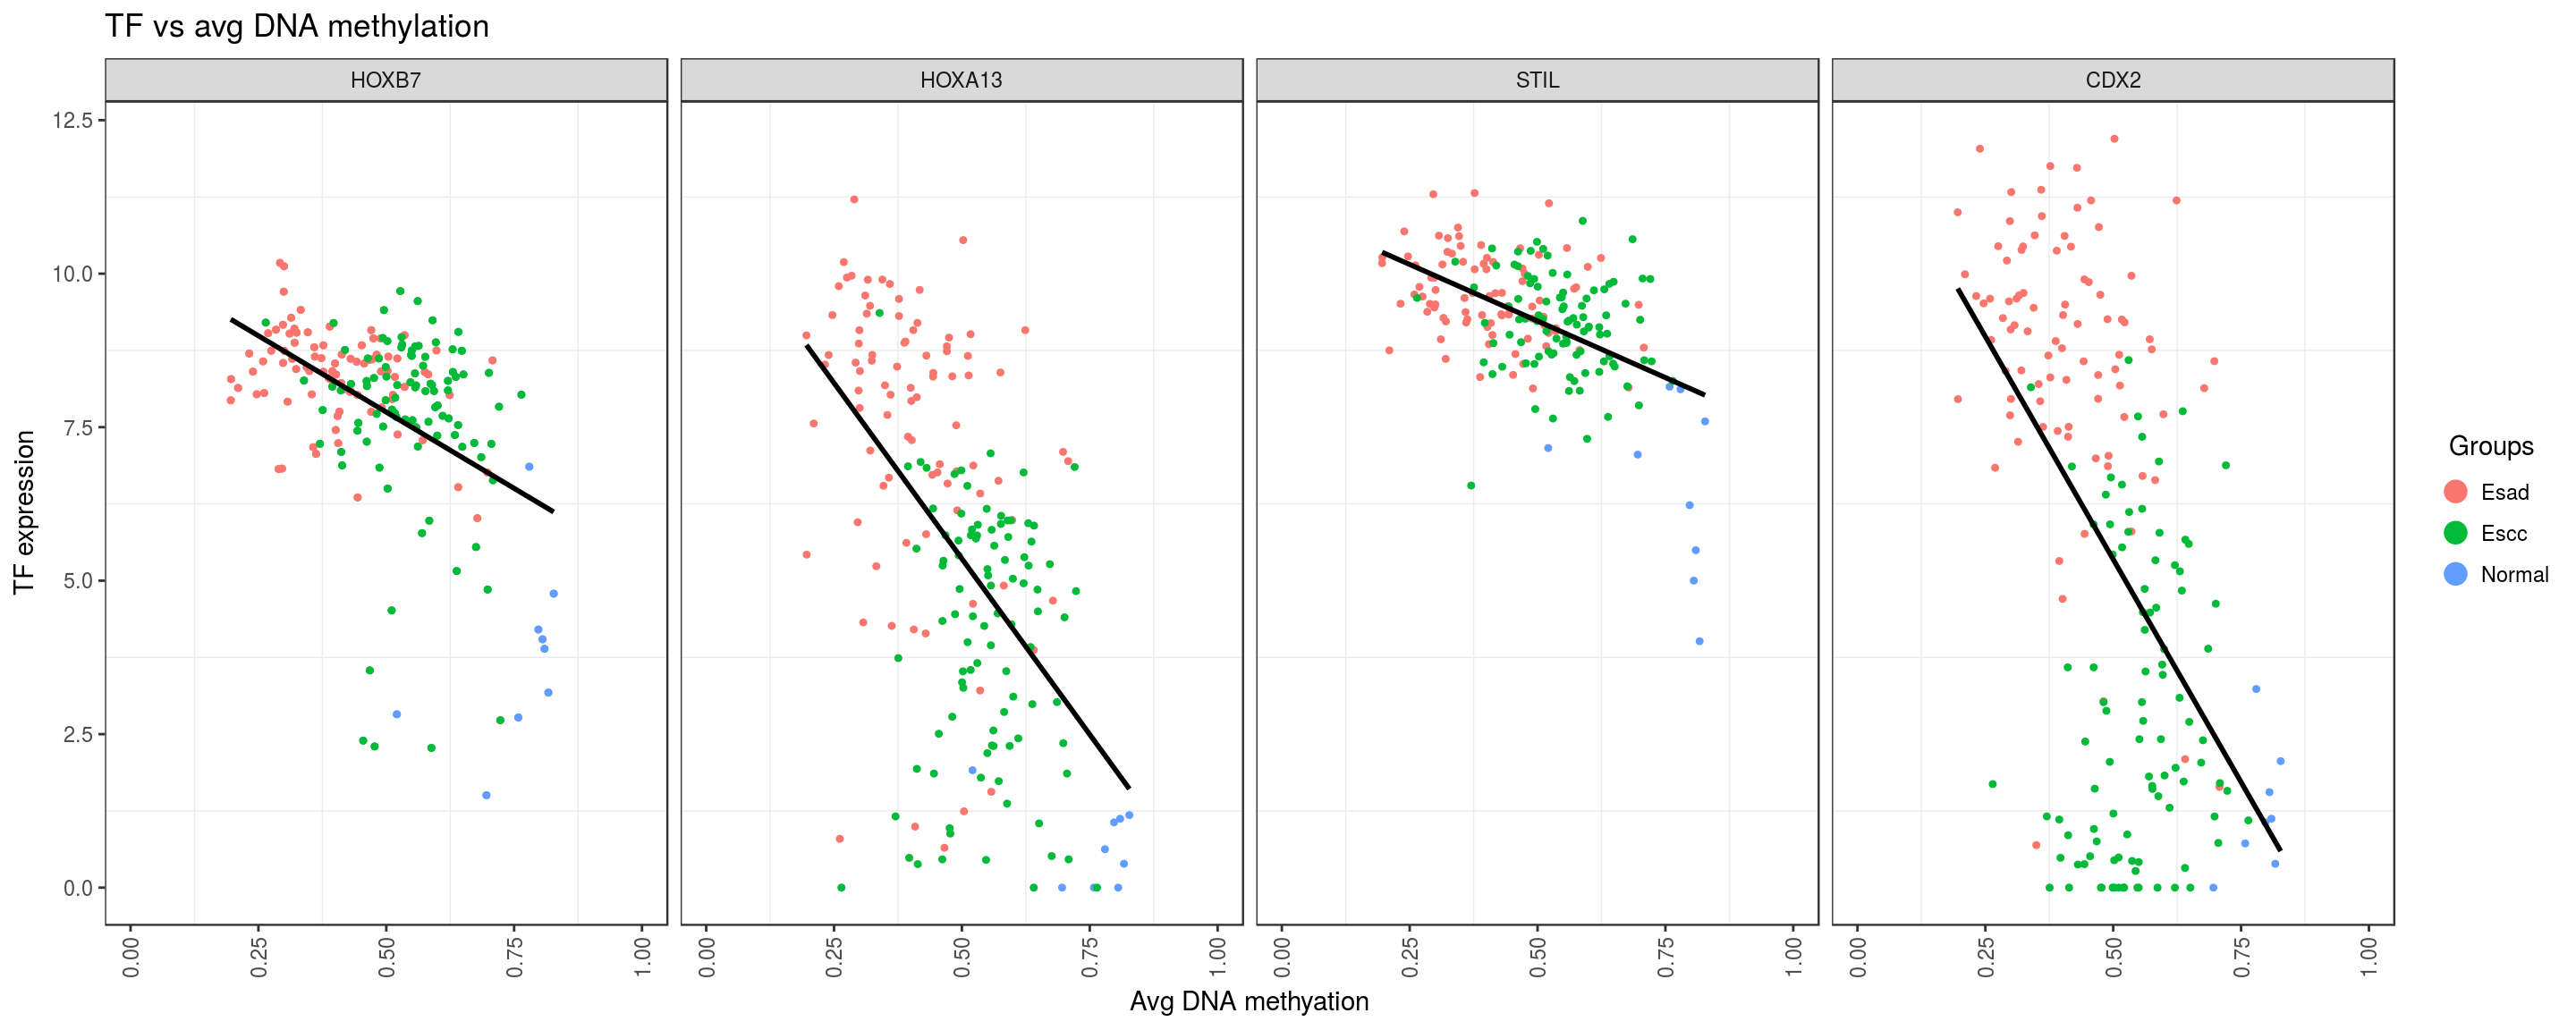
\includegraphics[width=1.0\linewidth]{ELMER/TF_plot_scatter.png}{\tiny{\\HOXB13 motif - Probes hypomethylated in esad vs normal}}
 \end{figure}
\end{frame}

\begin{frame}{Step 5: TF master regulator table}
 \begin{figure}
  \centering
  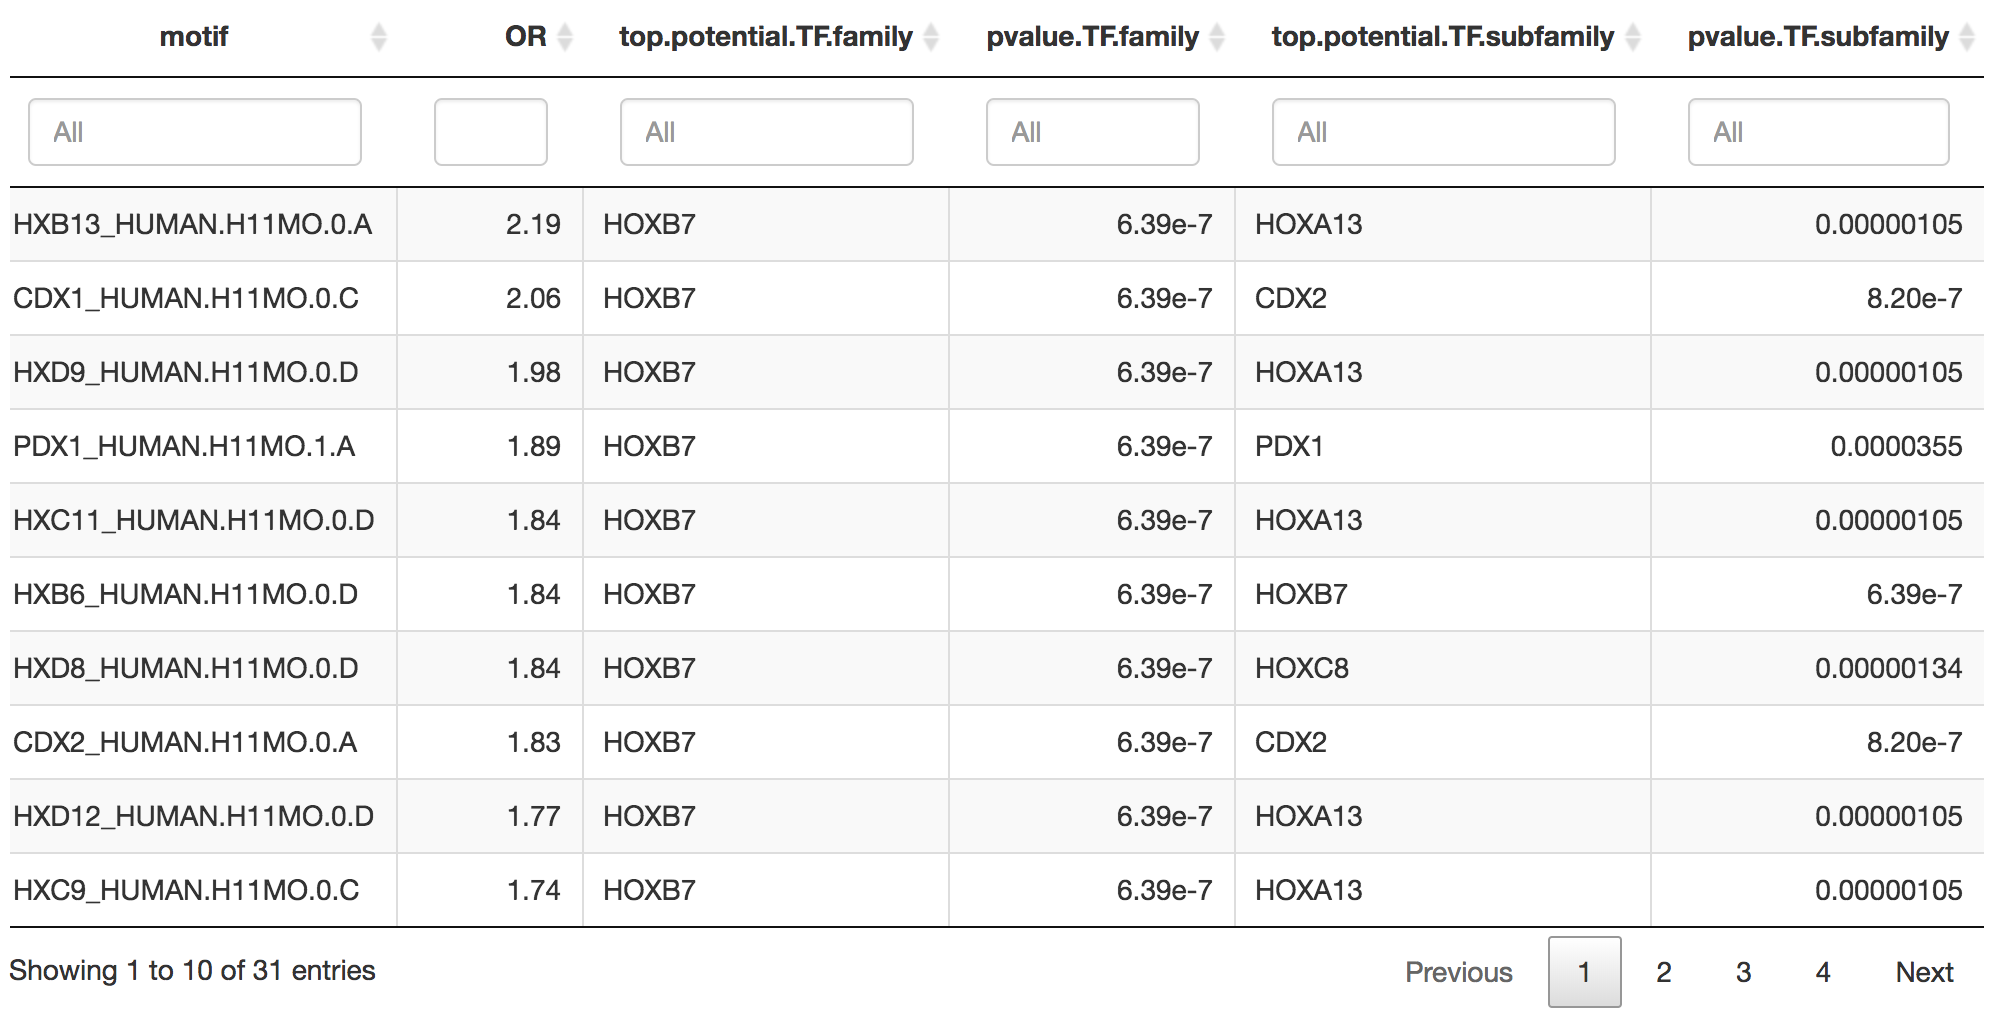
\includegraphics[width=1.0\linewidth]{ELMER/TF_tbl.png}
 \end{figure}
\end{frame}

\section{Comparison between versions}

\begin{frame}{Differences between versions}
 \tiny{
  \begin{table}[h!]
   \centering
   \caption{Main differences between ELMER version 1 and 2)}
   \label{tab:summary}
   \begin{tabular}{@{}p{2.5cm}p{3.5cm}p{4cm}@{}}
    \toprule
    \multicolumn{1}{c}{\textbf{Features}} & \multicolumn{1}{c}{\textbf{ELMER Version 1}} & \multicolumn{1}{c}{\textbf{ELMER Version 2}}               \\ \midrule
    Main data structure                   & mee object (own data structure)              & MAE object (Bioconductor data structure)                   \\
    Auxiliary data                        & Manually created                             & Programmatically created                                   \\
    Number of human TF                    & 1,982                                        & 1,987 (Uniprot database                                    \\
    Number of TF motifs                   & 91                                           & 771  (HOCOMOCO v11 database)                               \\
    TF classification                     & 78 families                                  & 80 families and 308 subfamilies \newline(TFClass database) \\
    Analysis performed                    & Normal tumor samples vs experiment           & Group 1 vs group 2                                         \\
    TCGA samples source                   & The Cancer Genome Atlas (TCGA)               & The NCI's Genomic Data Commons (GDC)                       \\
    Genome of reference                   & GRCh37 (hg19)                                & GRCh37 (hg19)/GRCh38 (hg38)                                \\
    DNA methylation platforms             & HumanMethylation450                          & HumanMethylationEPIC / HumanMethylation450                 \\
    %Graphical User interface (GUI)        & None                                   & In TCGAbiolinksGUI                       \\
    \bottomrule
   \end{tabular}
  \end{table}
 }
\end{frame}


\section{Case of study - TCGA BRCA}


\begin{frame}{TCGA Breast Invasive Carcinoma (BRCA) Samples}
 \begin{table}[ht!]
  \centering
  \caption{Summary of the available samples in TCGA for BRCA}
  \scriptsize

  \begin{tabular}{p{2.3cm}p{2.4cm}p{2.4cm}p{1cm}}
   \toprule
   Group               & Samples w/ DNA methylation (450K) & Samples w/ gene expression (FPKM-UQ) & Samples w/ both \\ \midrule
   Primary solid Tumor & 791                               & 1102                                 & 778             \\
   Solid Tissue Normal & 96                                & 113                                  & 83              \\
   \bottomrule
  \end{tabular}
 \end{table}

 \begin{table}[ht!]
  \centering
  \caption{Results}
  \scriptsize

  \begin{tabular}{p{2.8cm}p{2.4cm}}
   \toprule
   Inferred gene-probe pairs & 2167 \\
   Enriched motifs           & 312  \\
   Regulatory TF factors     & 17   \\
   \bottomrule
  \end{tabular}
 \end{table}
\end{frame}


\begin{frame}{Step 3: Pairs inferred}
 \vspace*{0.8cm}
 \begin{columns}[T]
  \begin{column}{0.5\textwidth}
   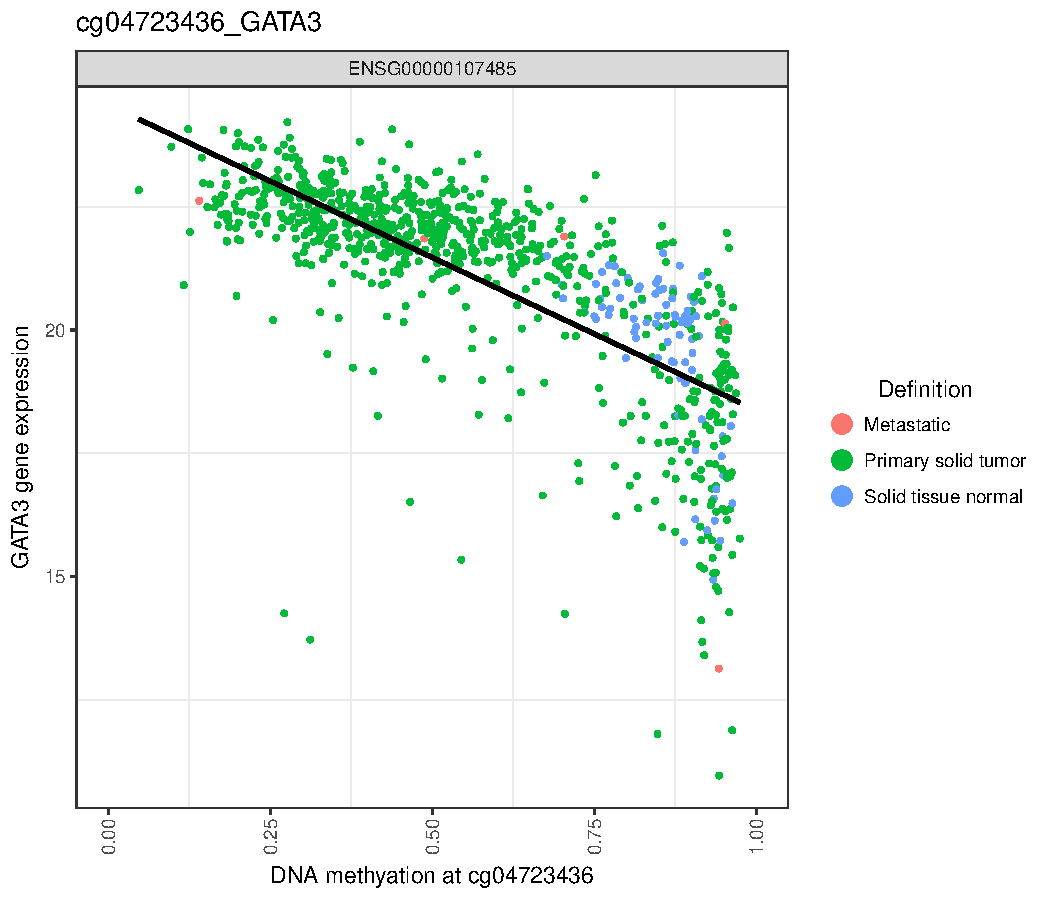
\includegraphics[width=1.0\linewidth]{cg04723436_GATA3_bypair.pdf}
  \end{column}
  \begin{column}{0.5\textwidth}
   \vspace{0.2cm}
   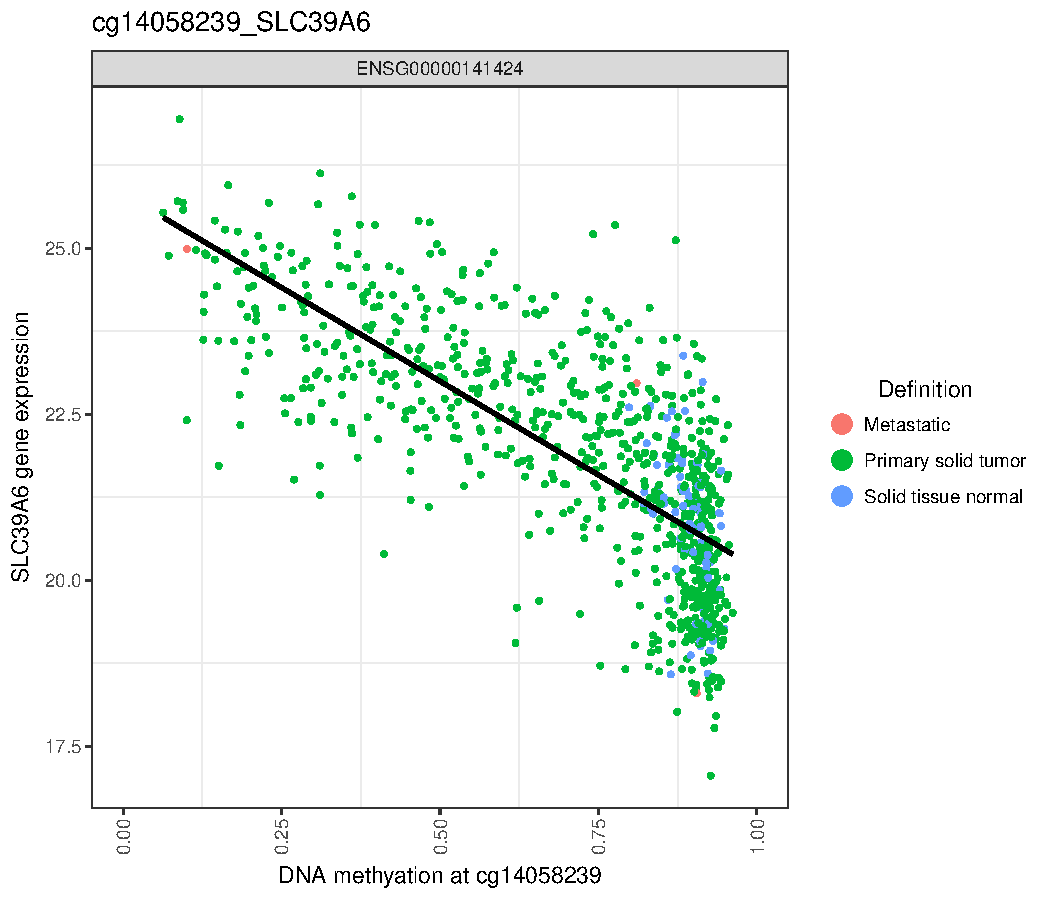
\includegraphics[width=1.0\linewidth]{cg14058239_SLC39A6_bypair.pdf}
  \end{column}
 \end{columns}
\end{frame}


\begin{frame}{Top enriched motifs}
 \vspace*{-0.3cm}
 \begin{figure}
  \centering
  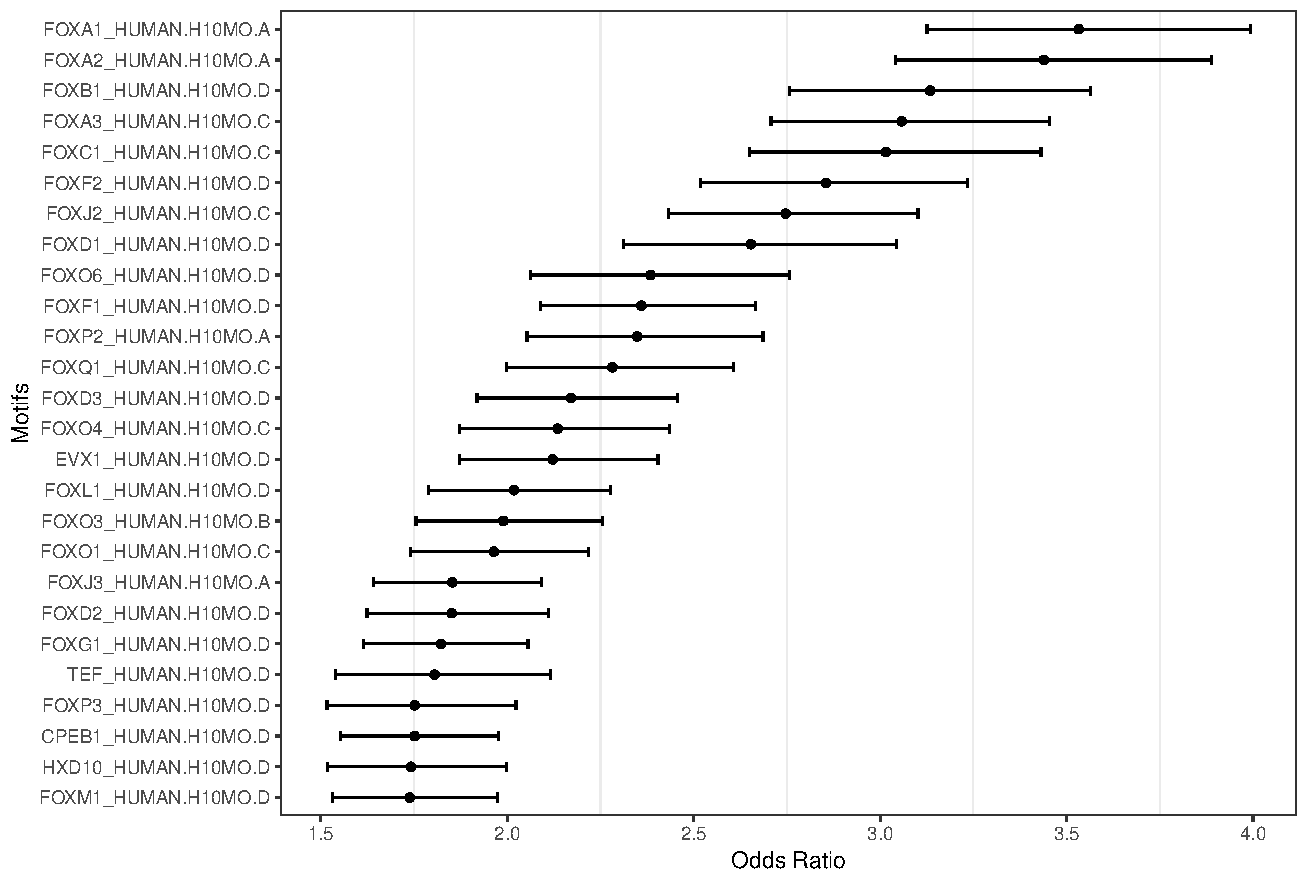
\includegraphics[width=1.0\linewidth]{ELMER/Motif_top.pdf}
 \end{figure}
\end{frame}

\begin{frame}{TF ranking}
 \vspace*{-0.3cm}
 \begin{figure}
  \centering
  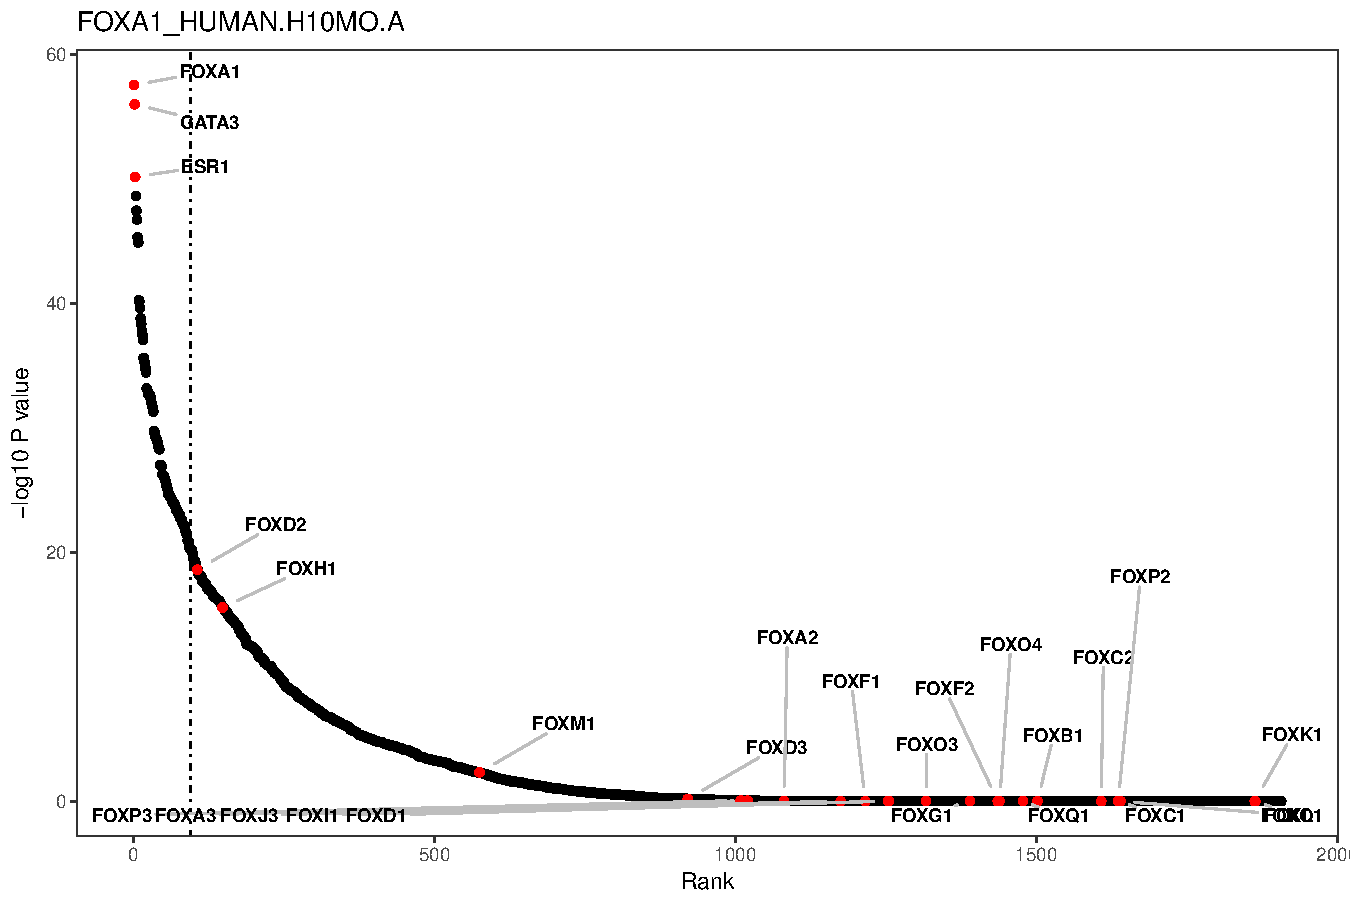
\includegraphics[width=1.0\linewidth]{ELMER/TF_FOXA1.pdf}
 \end{figure}
\end{frame}

\begin{frame}{Regulatory TF}
 \vspace*{-0.3cm}
 \begin{figure}
  \centering
  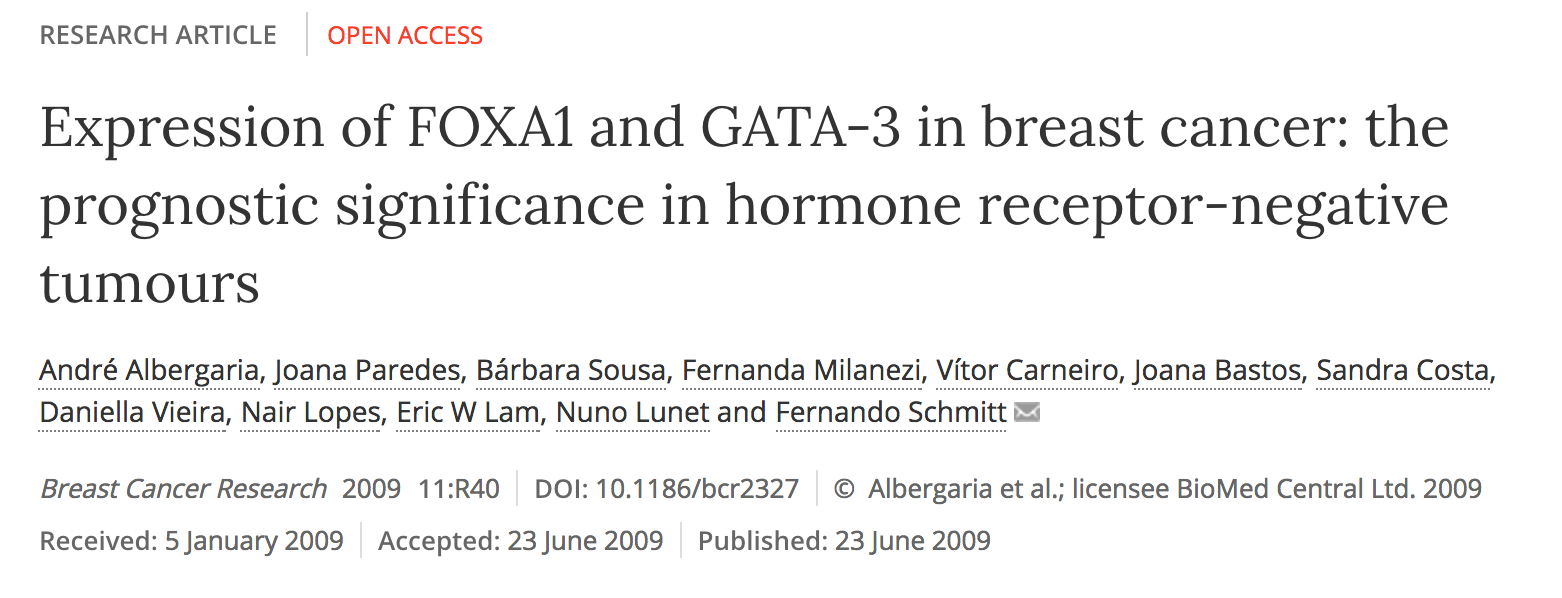
\includegraphics[width=0.8\linewidth]{ELMER/paper4.png}\\
  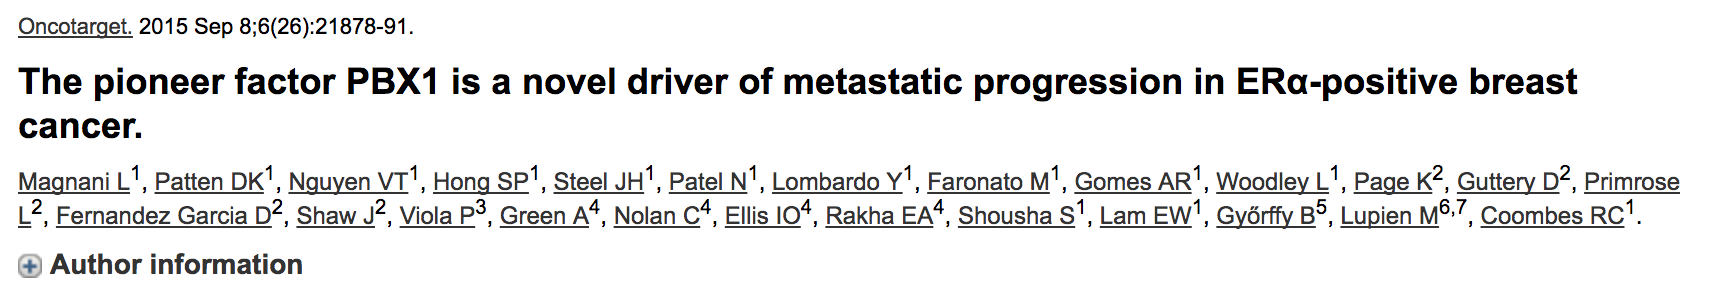
\includegraphics[width=0.8\linewidth]{ELMER/paper1.png}\\
  
\includegraphics[width=0.8\linewidth]{ELMER/paper2.png}
  %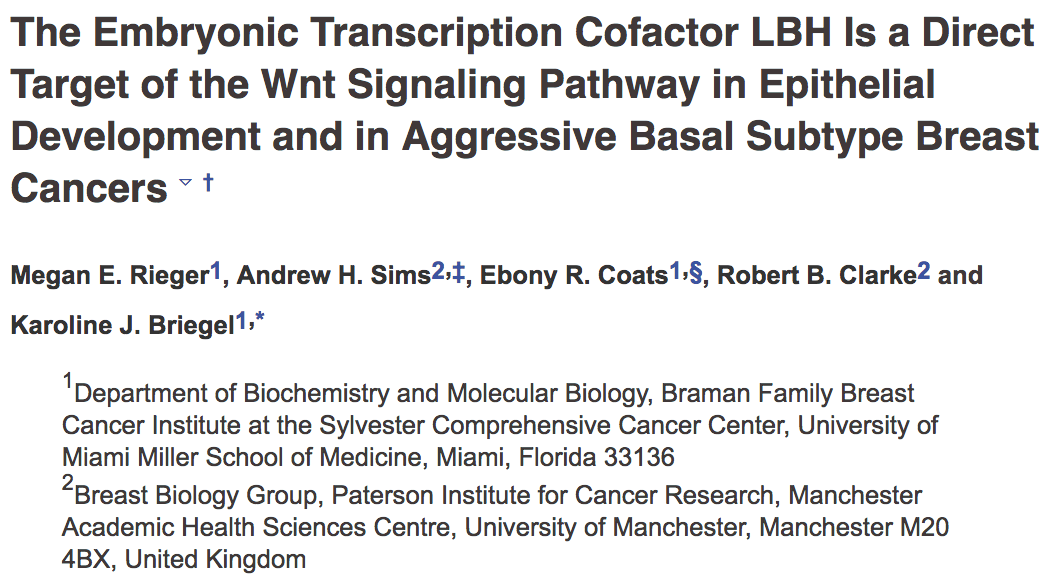
\includegraphics[width=0.8\linewidth]{paper3.png}
 \end{figure}
\end{frame}

\begin{frame}{Annotating chromatin state and verifying enrichment}
 \vspace*{-0.3cm}
 \begin{figure}[ht!]
  \centering
  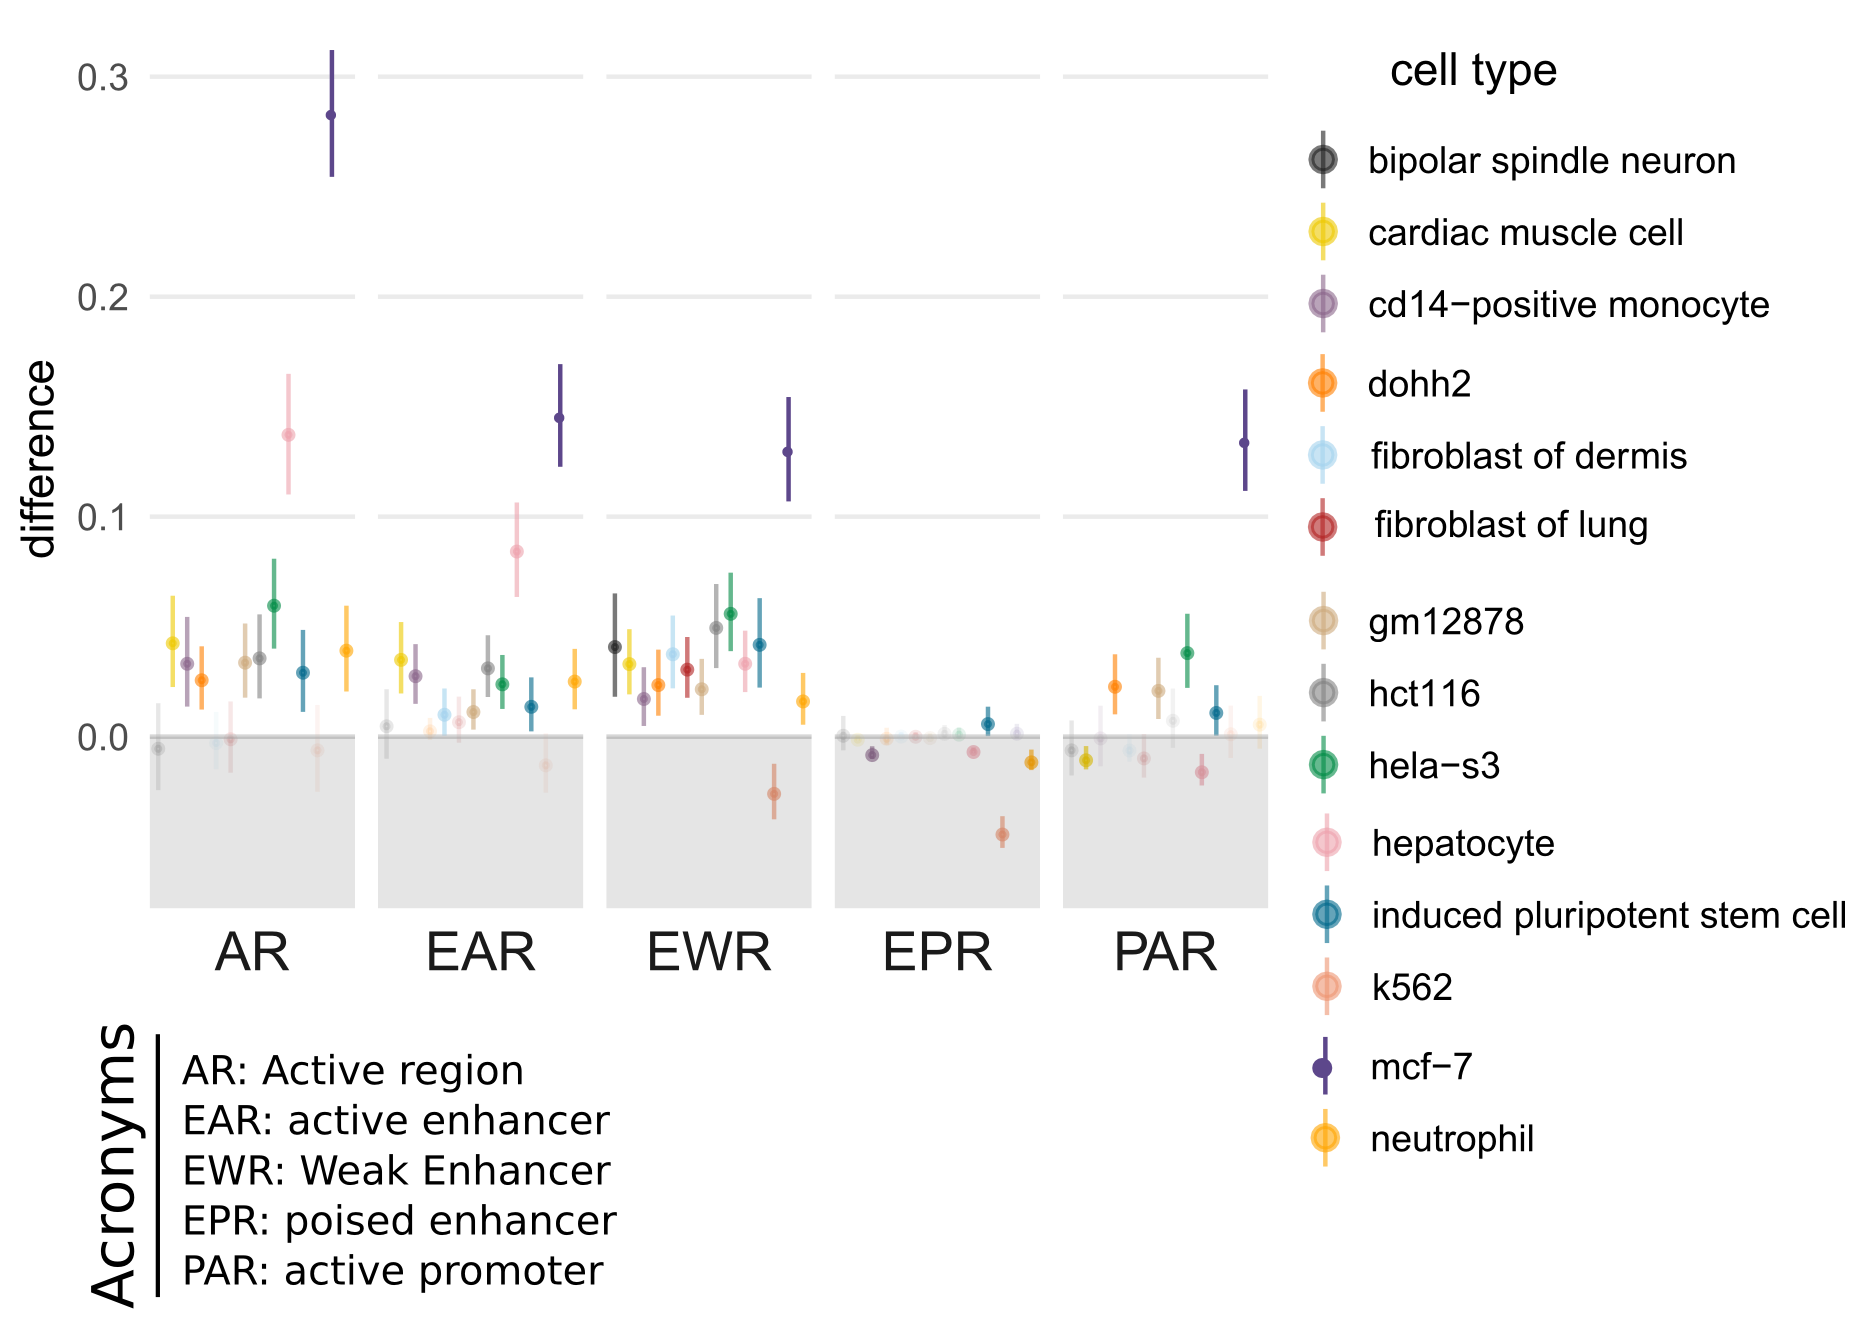
\includegraphics[width=0.9\textwidth]{images/1.png}%\tiny{\\Enrichment of paired probes and chromatin states of encode cells. The plot shows enrichment for enhancer active region (EAR), weak enhancer (EWR) and active promoter region (PAR) for MCF-7 cell. }
 \end{figure}
 \pdfnote{remember to say thank you to simon}
 \pdfnote{
  Enrichment of paired probes and chromatin states of encode cells. The plot shows enrichment for enhancer active region (EAR), weak enhancer (EWR) and active promoter region (PAR) for MCF-7 cell.
  Acronyms - AR: Active region, EAR: active enhancer, EWR: Weak Enhancer, EPR: poised enhancer, PAR: active promoter, PWR: Weak Promoter, PPR: poised promoter, PPWR: Weak Poised Promoter, CTCF: architectural complex, TRS: transcribed, HET: heterochromatin, SCR: Polycomb Repressed Silenced
 }
\end{frame}

\begin{frame}{Comparing inferred results with MCF-7 chIA-PET}

 \begin{figure}[ht!]
  \centering
  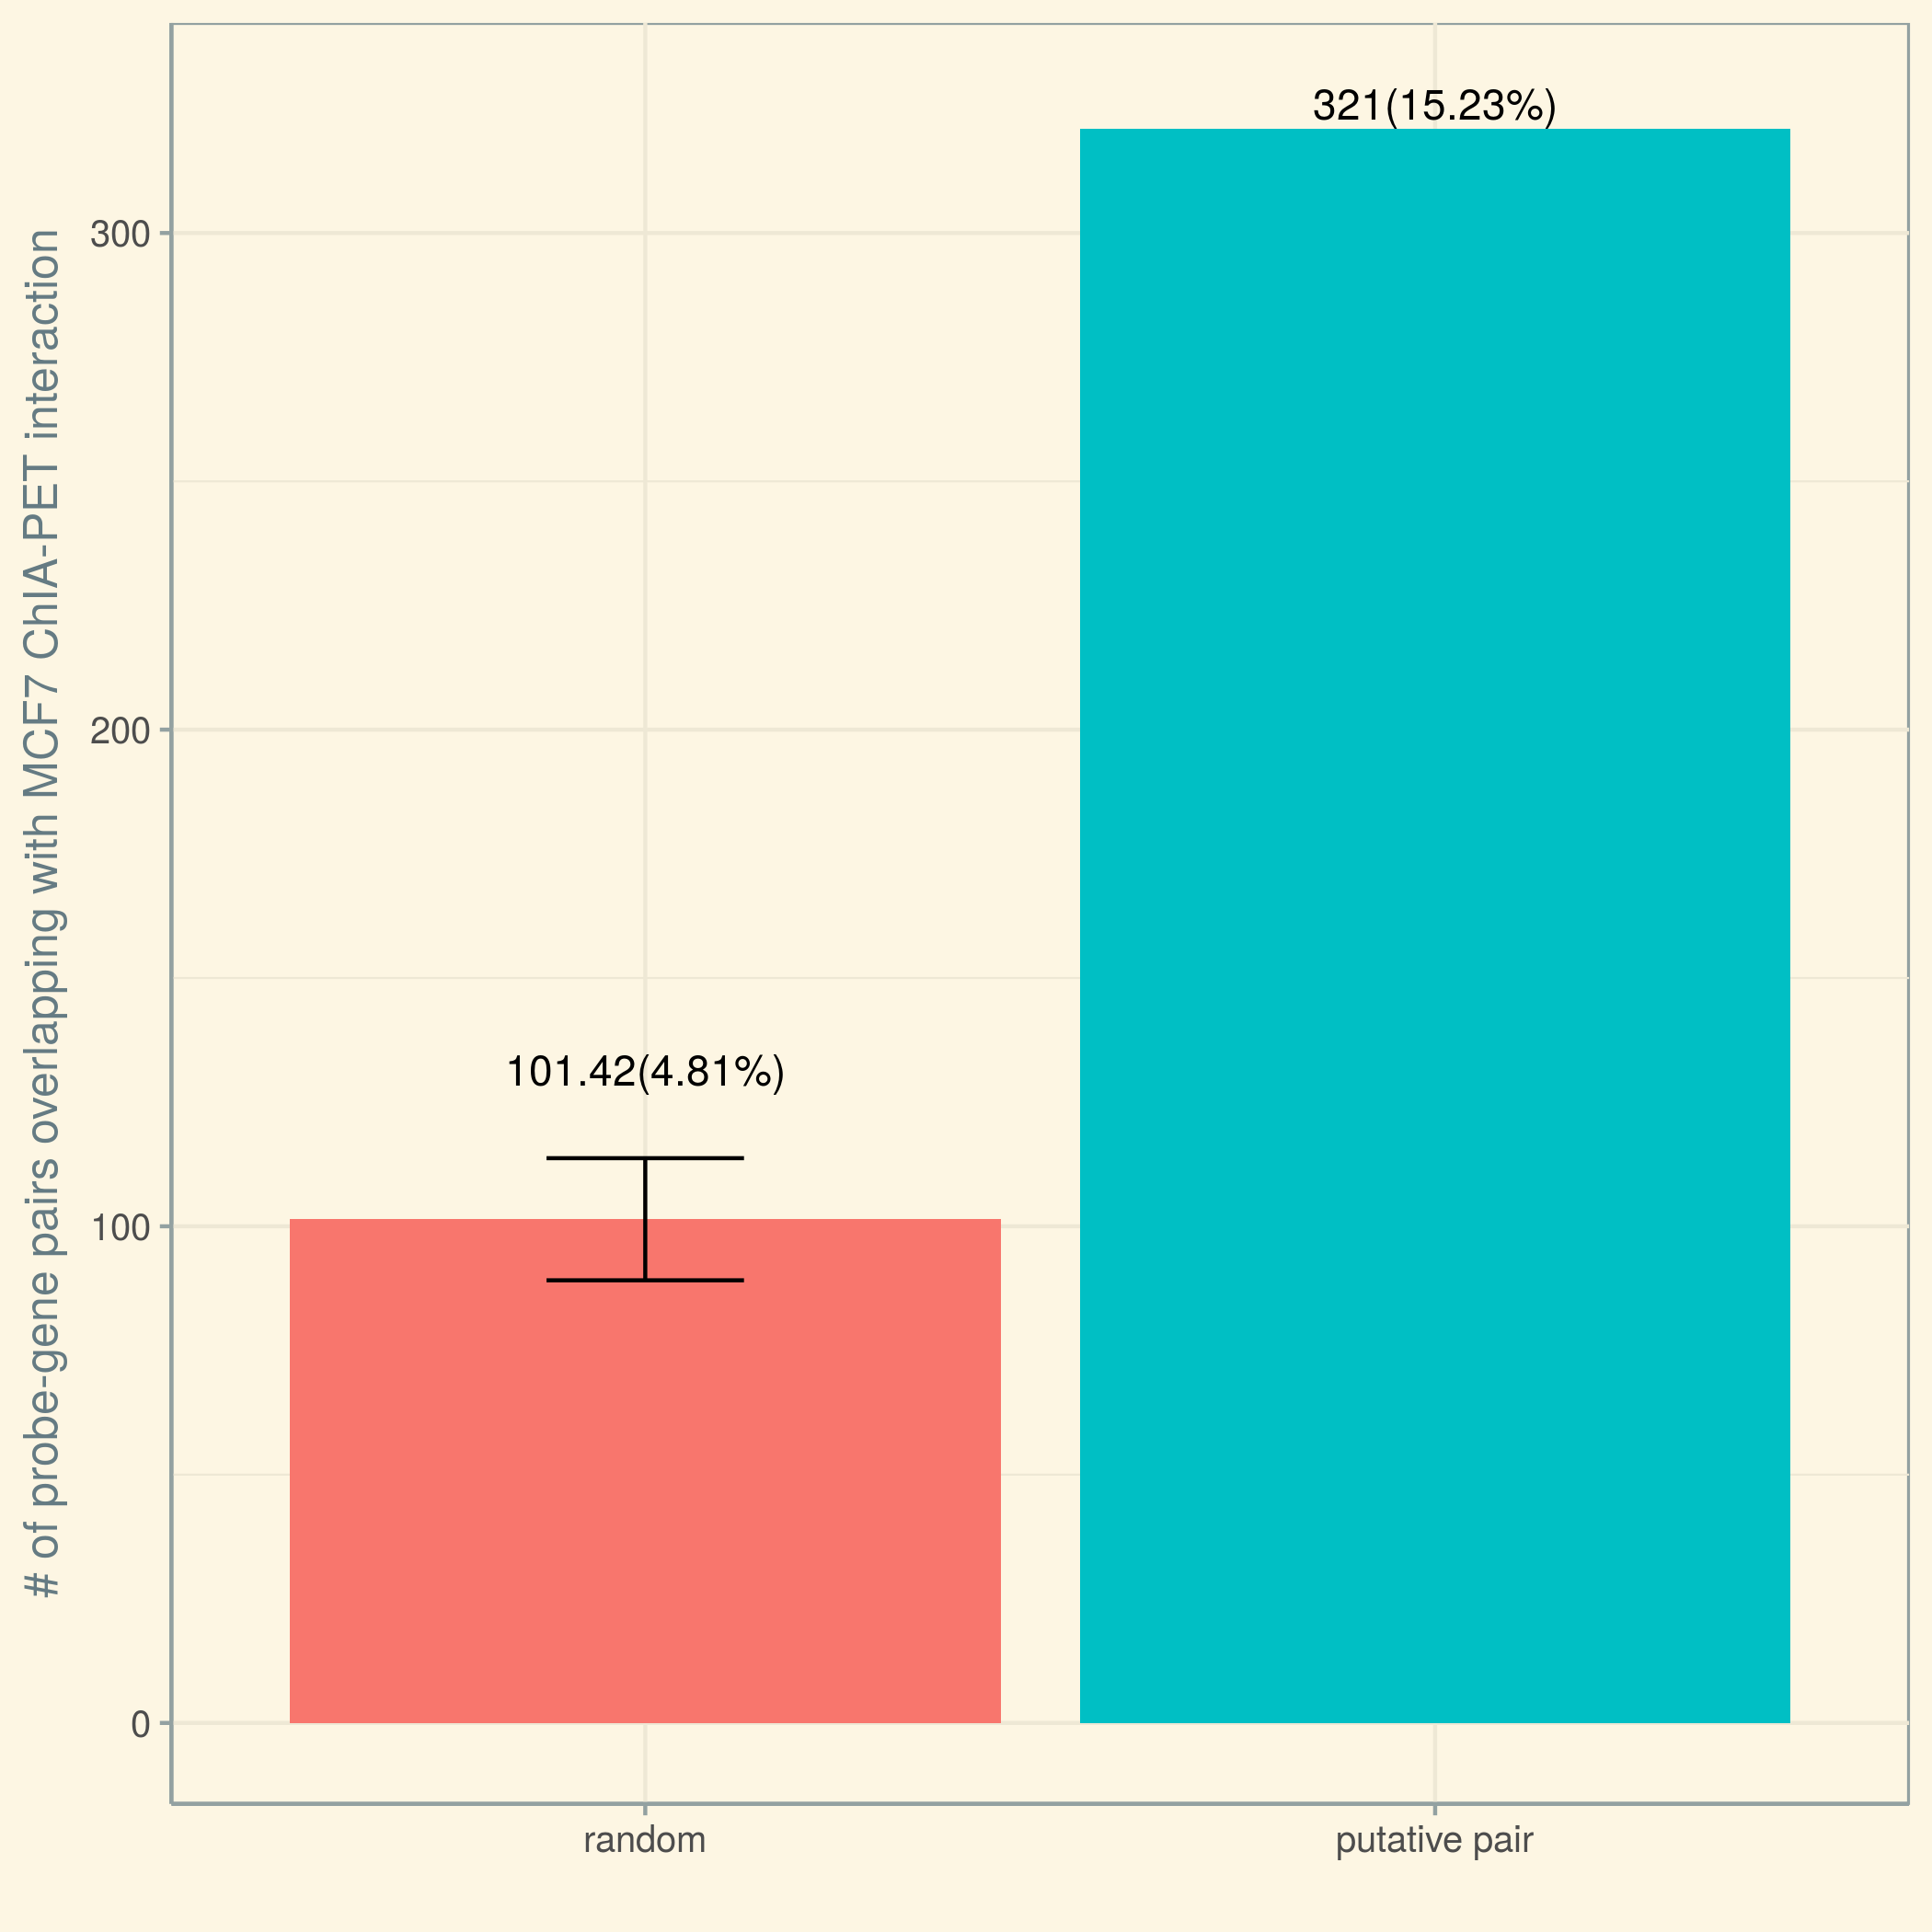
\includegraphics[width=0.6\textwidth]{ELMER/validation.png}
  \caption{\label{fig:chiapet} The graph shows the comparison of the number of probe-gene pairs identified within MCF7 ChIA-PET data using the putative pairs from BRCA vs. random pairs}
 \end{figure}
\end{frame}



\begin{frame}{Acknowledgments}
 %\vspace{-0.5cm}
 \begin{columns}[T]
  \begin{column}{0.5\textwidth}
   \begin{block}{University of São Paulo}
    \begin{itemize}
     \item  Houtan Noushmerh
    \end{itemize}
   \end{block}
  \end{column}
  \begin{column}{0.5\textwidth}
   \vspace{0.2cm}
   
\includegraphics[width=0.4\linewidth]{logo/usp.png}
  \end{column}
 \end{columns}

 \vspace{0.2cm}
 \begin{columns}[T]
  \begin{column}{0.5\textwidth}
   \begin{block}{Cedars-Sinai}
    \begin{itemize}
     \item Ben Berman
     \item Simon Coetzee
     \item Dennis Hazelett
     \item Nicole Yeager
     \item Huy Dinh
     \item Michelle Jones
     \item Alberto Reyes
     \item Ivetth Corona
    \end{itemize}
   \end{block}
  \end{column}
  \begin{column}{0.5\textwidth}
   \vspace{2.5cm}
   
\includegraphics[width=1.0\linewidth]{cedars.png}
  \end{column}
 \end{columns}

\end{frame}


\begin{frame}{References}
 \begin{thebibliography}{10}
  \tiny
  \beamertemplatebookbibitems
  \bibitem{Oppenheim2009}
  Ginsburg, Geoffrey S., and Huntington F. Willard.
  \newblock Genomic and personalized medicine.
  \newblock  Vol. 1. Academic Press, 2008.

  \beamertemplatearticlebibitems
  \bibitem{F10002016}
  Silva TC, Colaprico A, Olsen C et al.
  \newblock TCGA Workflow: Analyze cancer genomics and epigenomics data using Bioconductor packages
  \newblock  F1000Research 2016, 5:1542

  \beamertemplatearticlebibitems
  \bibitem{EBU2011}
  H. Noushmehr, D. J. Weisenberger, et al.
  \newblock Identification of a CpG island methylator phenotype that defines a distinct subgroup of glioma.
  \newblock Cancer Cell, 17(5):510–522, May 2010.

  \beamertemplatearticlebibitems
  \bibitem{EBU2011}
  S. Sharma, T. K. Kelly, and P. A. Jones.
  \newblock Epigenetics in cancer.
  \newblock  Carcinogenesis, 31(1):27–36, Jan 2010.

  \beamertemplatearticlebibitems
  \bibitem{EBU2011}
  Tiago Chedraoui Silva*, Antonio Colaprico*, et al.
  \newblock TCGAbiolinks: An R/Bioconductor package for integrative analysis of TCGA data. Nucleic Acids Res.,
  \newblock Nucleic acids research, p.gkv1507, 2015

  \beamertemplatearticlebibitems
  \bibitem{EBU2011}
  Ceccarelli M, Barthel FP, Malta TM, Sabedot TS, Salama SR, et al. . Cell,
  \newblock Molecular profiling reveals biologically discrete subsets and pathways of progression in diffuse glioma
  \newblock Cell, 164(3):550-563, 2016


  %	\beamertemplatearticlebibitems
  %	\bibitem{EBU2011}
  %S. B. Baylin and P. A. Jones.
  %	\newblock A decade of exploring the cancer epigenome - biological and translational implications.
  %	\newblock Nat. Rev. Cancer, 11(10):726–734, Oct 2011.

 \end{thebibliography}
\end{frame}


\begin{frame}{Thank you for your attention!}
 \vspace*{2.5cm}
 \centering
 \Huge{Any questions?}
\end{frame}

%-=-=-=-=-=-=-=-=-=-=-=-=-=-=-=-=-=-=-=-=-=-=-=-=
%
%	SECTION: Conclusion
%
%-=-=-=-=-=-=-=-=-=-=-=-=-=-=-=-=-=-=-=-=-=-=-=-=


\end{document}
